\chapter{The Deep Learning Approach}\label{mlChapter}

This chapter describes and analyses a novel approach to the specific problem of
chess puzzle classification, inspired by the recent unstoppable advancements in
the field of natural language processing.

The justification for why transformers may work, along with a slightly more
formal problem statement, is outlined (\Cref{mlS0}).

The data pipeline is then discussed (\Cref{mlS1}), starting with the bitboard
encoding (\Cref{mlS11}) and ending with the training, validation, and testing
splits (\Cref{mlS12}).

The process of creating the model is then described in detail (\Cref{mlS2}),
including architecture (\Cref{mlS21}), training setup (\Cref{mlS23}), and
hyperparameter selection (\Cref{mlS22}).

Finally, the internals of the model are explored (\Cref{mlS3}) by visualising
the input for specific chess boards (\Cref{mlS32}). These are then discussed
(\Cref{mlS33}).


\section{Overview}\label{mlS0}

\subsection{Why Should This Work?}

Earlier (\Cref{bg4}), some papers were highlighted which seek to find new ways
to build on the naive bitboard representation by exploring new embeddings for
chess pieces and chess board squares. These publications make the crucial point
that chess pieces influence each other on the board, and this has to be taken
into account, whether it is by creating extra features to represent pins and
central square control \citep{chessCNN}, open files and attack squares
\citep{middleGamePatterns}, or the hash of the entire chess board
\cite{chess2vec}.

Continuing along the `chess board as a $N\times64$ vector' path and, given how
puzzle tactics rely on the interaction of pieces' locations and attack squares,
it seems natural to explore whether the transformer architecture, as described
in the infamous paper `Attention Is All You Need' by \citet{attention}, can
help extract patterns from static chess positions, which can then be used in
the downstream task of puzzle classification and difficulty rating. A
correspondence can be drawn between how words/tokens influence each other in
the transformer encoder (\Cref{attentionLinks}) and how chess pieces/squares
interact on the 64 squares (\Cref{chessPuzzleLinks}).

Applying transformers to chess has been done before by
\citet{chessTransformer}, whose work is reviewed at the end of the report
(\Cref{chessTransformerSection}), but treating individual chess board squares
as embeddings of tokens/words has not been previously explored.

\begin{figure}[H]
  \begin{minipage}{0.4\textwidth}
    \centering
    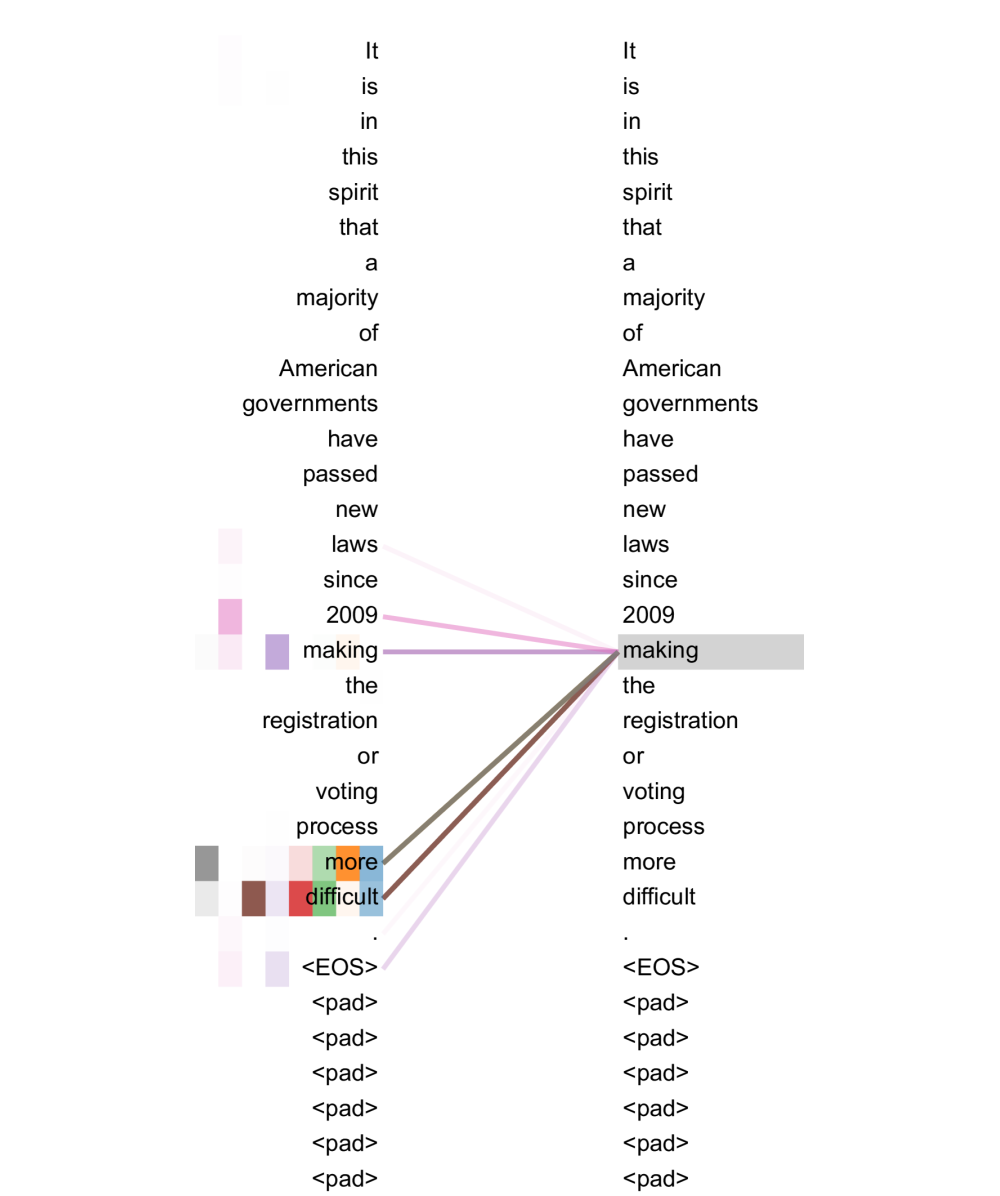
\includegraphics[width=\textwidth]{project/img/attention.png}
    \caption{Example of the attention mechanism in the encoder. Taken from
    `Attention Is All You Need' \citep{attention}.}
    \label{attentionLinks}
  \end{minipage}
  \hspace{0.05\textwidth}
  \begin{minipage}{0.475\textwidth}
    \centering
    \chessboard[setfen=r3r1n1/bp6/p2p2kp/3N4/2P3n1/1PQ3Pq/P4P2/4RRK1 w - - 0 1,
    pgfstyle=border,markfields={d5},
    pgfstyle=straightmove,
    markmoves={f4-g6,f4-h3,c7-a8,c7-e8,d5-c7,d5-f4},
    pgfstyle=color,opacity=0.5,
    color=blue,markfields={f4,c7},
    pgfstyle=color,opacity=0.5,
    color=red,markfields={h3,g6,a8,e8}]

    \caption{Example of a relationship between chess pieces and squares.}

    \label{chessPuzzleLinks}
  \end{minipage}
\end{figure}

\subsection{Problem Statement}

Given a dataset with $N$ distinct puzzle labels ($N=60$ for the Lichess puzzle
database), each label is assigned an index $i$ and a binary $N$-dimensional
vector $x$ is formed such that $x[i]=1$ iff the puzzle is labelled with that
label. This is a common technique to reduce a multi-label classification into a
more tractable problem.

With this, a model is to be developed that, given a stationary chess position
in FEN (\Cref{fenSection}), returns a prediction for this
position's puzzle label vector.

\section{The Data}\label{mlS1}

\subsection{Bitboard Encoding}\label{mlS11}

The string-based FEN is naturally incompatible for machine learning models. To
solve this, $12\times8\times8$ chess bitboards are used, which was also seen in
the work of \citet{chess2vec}. Slightly more formally, the element $B[z, x, y]$
of bitboard $B$ is $1$ iff there is a piece $z \in \{\texttt{p}, \texttt{P},
\texttt{n}, \texttt{N}, \texttt{b}, \texttt{B}, \texttt{r}, \texttt{R},
\texttt{q}, \texttt{Q}, \texttt{k}, \texttt{K}\}$\footnote{FEN-inspired --
white pieces are uppercase, black pieces are lowercase.} at rank $x \in
\{\texttt{1}, \texttt{2}, \texttt{3}, \texttt{4}, \texttt{5}, \texttt{6},
\texttt{7}, \texttt{8}\}$}, file $y \in \{\texttt{a}, \texttt{b}, \texttt{c},
\texttt{d}, \texttt{e}, \texttt{f}, \texttt{g}, \texttt{h}\}$.

This method has 2 major downsides: there is no way to distinguish if en passant
or castling is legal. However, there are only 5644 (0.14\%) puzzles tagged as
`en passant' in the Lichess database, and 2029 (0.053\%) tagged as `castling'
-- this is a negligible number and the rare situations where a tactic would be
changed by an impossible en passant/castle being possible can be ignored.

To make learning easier (and to decrease implementation complexity), all chess
positions are transformed to be from the perspective of White. This has
negligible additional overhead, as it requires a simple mirror and has great
benefits, as the model no longer needs to distinguish between White-to-move and
Black-to-move puzzles.

\subsection{Train/Validation/Test Split}\label{mlS12}

As is standard in statistical learning problems, the dataset is split into 3
non-overlapping subsets: a training set containing 60\% of the data, a
validation set containing 20\% of the data, and a test set with the remaining
20\% of the data. The training set is used to train the model, the validation
set is used to find the optimal set of hyperparameters (\Cref{mlS22}), and the
test set is withheld until the final evaluation section to get an estimate of
the model's performance on unseen data. 

\section{The Model}\label{mlS2}

\subsection{Architecture}\label{mlS21}

The overview of the model architecture is shown in \Cref{MLDiagram}. 

At first, there is a pointwise convolution to expand the 12 piece bitboards to
64 channels. This is followed by a stack of `embedding layers'. Each embedding
layer consists of an $8\times8$ convolution with circular padding, to allow
every chess square access to other chess squares. The channel count is kept
constant within every embedding layer. Between each of the four embedding
layers lies a pointwise convolution which doubles the channel count. The number
of layers and layer channels are defined at the creation of the model and are
optimised during the hyperparameter search stage (\Cref{mlS22}). Every
convolution layer is followed by the rectified linear unit (ReLU) activation
and batch normalisation \citep{ioffe2015batch}.

This embeds the 64 chess squares in a 512-dimensional space. The 2D structure
of the board is flattened, and passed through 8 standard transformer encoder
\citep{attention} layers, featuring self-attention and a feedforward layer. The
internal dropout and activation of the transformer encoder layer was kept
default (0.1 and ReLU, respectively). The feedforward layer size was optimised
(\Cref{mlS22}).

Finally, the entire output is flattened and a fully connected layer connects
this to the 60 output neurons, which correspond to each of the 60 Lichess
puzzle database themes. As the themes are not mutually exclusive, softmax
cannot be used, so sigmoid activation is used to map the outputs to the range
to $(0, 1)$.

\begin{figure}[H]
  \centering
  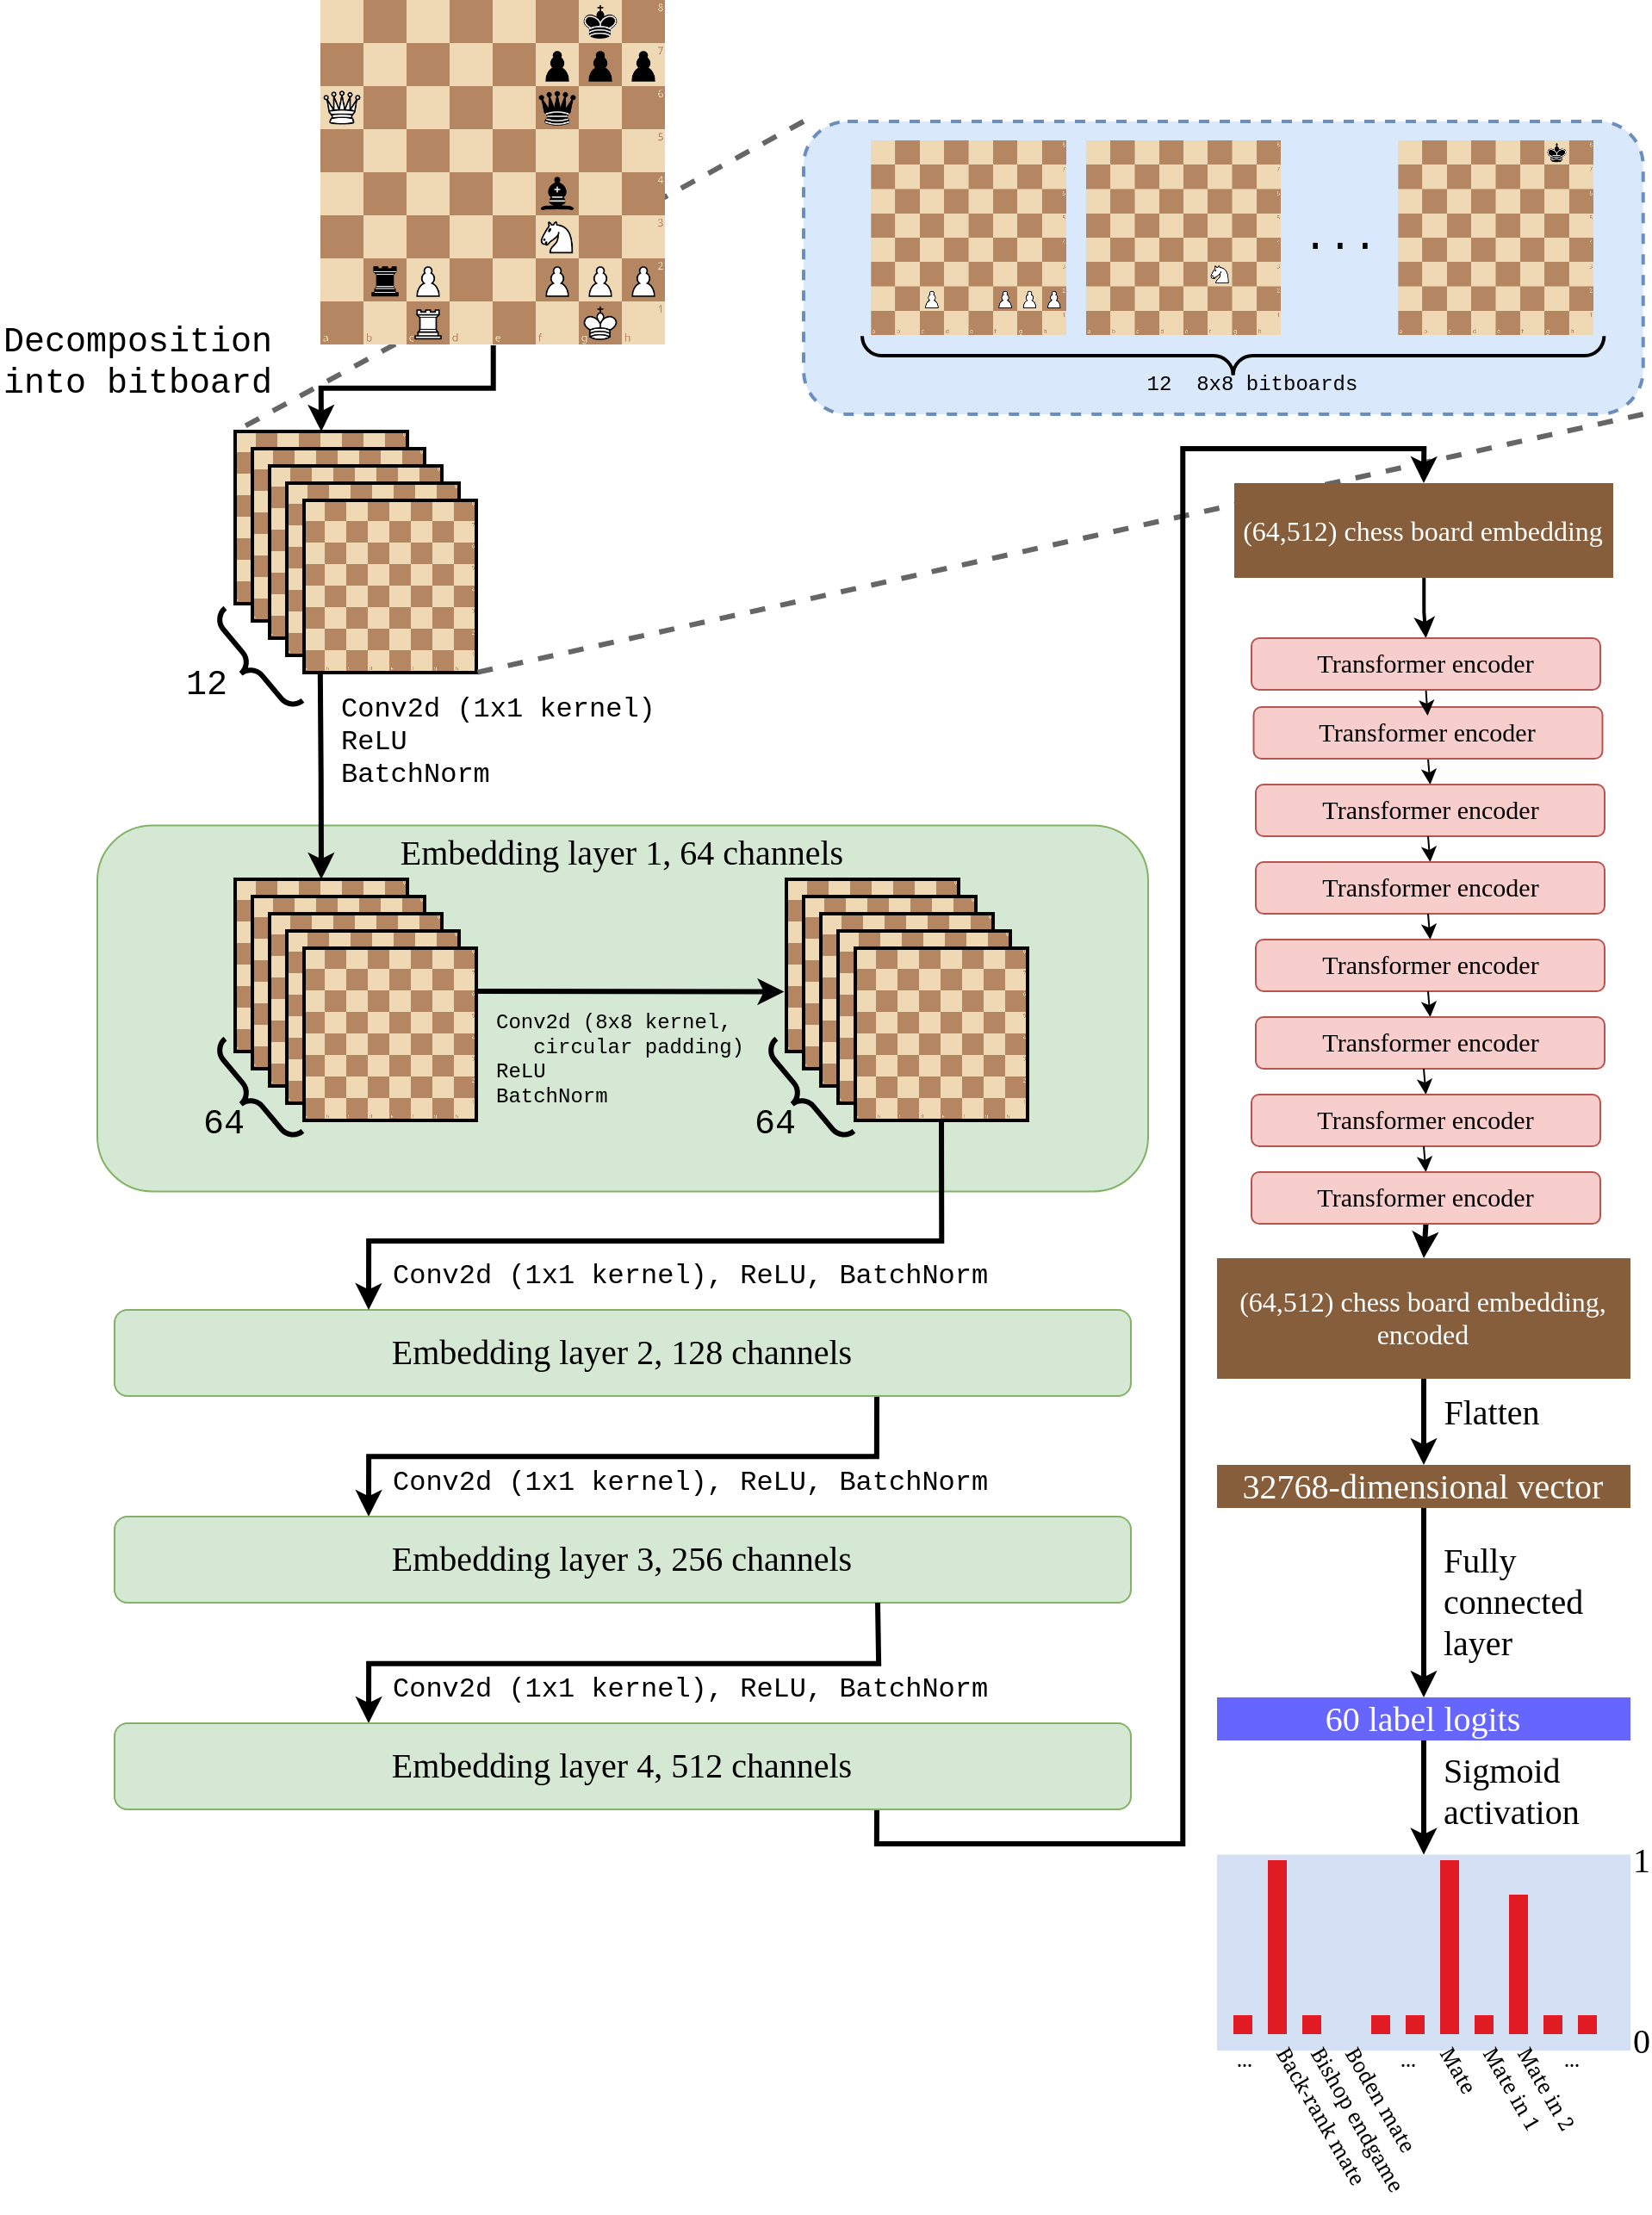
\includegraphics[width=0.55\textwidth]{project/img/ml_diagram.png}
  \caption{High-level overview of the model architecture.}
  \label{MLDiagram}
\end{figure}

\subsection{Training Setup}\label{mlS23}

The model was trained for 5 epochs. The data was batched into batches of size
128, and the average binary cross-entropy loss (\Cref{bceEq}) between the
expected labels and the predicted labels was used as the target to be
minimised. The Adam optimiser \citep{kingma2014adam}, an extension of
stochastic gradient descent, was used for weight updates, with a learning rate
of $1\times10^{-5}$ and default $\beta_1$, $\beta_2$.

\begin{equation}\label{bceEq}
  L(y, \hat{y}) = -\frac{1}{N}\sum_{i=0}^N \hat{y}_i \log y_i +
    (1-\hat{y}_i)\log(1-y_i)
\end{equation}

The model was trained on the Department of Computing's GPU Slurm Cluster,
managed by \citet{csgGPU}. This cluster contains a multitude of NVIDIA GPUs;
the cited website has an exhaustive list. Each epoch took approximately 1h-2h,
depending on resource availability and hyperparameter combination.

\subsection{Hyperparameters}\label{mlS22}

To find the optimal hyperparameters, a grid search was performed over a subset
of the hyperparameters (\Cref{tabHyperparam}). 

There is evidence of overfitting for the larger models with with $\sim\!33$
million parameters. These achieve a low training loss of approximately 0.08,
but the validation loss greatly suffers as a result. Overall, the
hyperparameter combination with the best performance on the validation set (row
is highlighted) was selected.

The loss curves for this model over the 5 epochs are shown (\Cref{lossCurves}).
While these do not show total convergence, the performance of the model was
adequate and to keep it fair for all combinations, no more training was done.

\begin{table}[H]
  \centering
  \begin{adjustbox}{width=\textwidth}
    \begin{tabular}{lll|rrr}

      \multicolumn{3}{c}{Hyperparameter} && \multicolumn{2}{c}{Average loss
      after 5 epochs} \\

      Embedding layer channels & \texttt{n\_heads} & \texttt{ff\_dim} & Total
      parameters & Train & Validation\\

      \hline

      $[64, 128, 256, 512 ]$& $32$ & $4096$ & 33,114,812 & 0.08161 & 0.1016   \\
      $[64, 128, 256, 512 ]$& $32$ & $8192$ & 33,114,812 & 0.08156 & 0.1011 \\
      $[64, 128, 256, 512 ]$& $32$ & $16384$ & 33,114,812 & 0.08092 & 0.09937 \\[0.1cm]

      $[64, 128, 256, 512 ]$& $64$ & $4096$ & 33,377,212 & 0.08089 & 0.1026 \\
      $[64, 128, 256, 512 ]$& $64$ & $8192$ & 33,377,212 & \textbf{0.08031} & 0.1019 \\ [0.5cm]

      $[32, 64, 128, 256 ]$& $32$ & $4096$ & 8,846,844 & 0.09416 & 0.09942 \\
      $[32, 64, 128, 256 ]$& $32$ & $8192$ & 8,846,844 & 0.09452 & 0.09991 \\
      $[32, 64, 128, 256 ]$& $32$ & $16384$ & 8,846,844 & 0.09442 & 0.09990 \\[0.1cm]

      $[32, 64, 128, 256 ]$& $64$ & $4096$ & 8,978,172 & 0.09424 & 0.09987 \\
      $[32, 64, 128, 256 ]$& $64$ & $8192$ & 8,978,172 & 0.09395 & 0.09990 \\
      $[32, 64, 128, 256 ]$& $64$ & $16384$ & 8,978,172 & 0.09425 & 0.1001 \\[0.1cm]

      $[32, 64, 128, 256 ]$& $128$ & $4096$ & 9,240,828 & 0.09351 & 0.09918 \\
      $[32, 64, 128, 256 ]$& $128$ & $8192$ & 9,240,828 & 0.09341 & 0.09953 \\
      $[32, 64, 128, 256 ]$& $128$ & $16384$ & 9,240,828 & 0.09387 & 0.09914 \\[0.5cm]

      $[64, 128, 256 ]$& $32$ & $4096$ & 8,779,452 & 0.09234 & 0.09823 \\
      $[64, 128, 256 ]$& $32$ & $8192$ & 8,779,452 & 0.09161 & 0.09787 \\
      $[64, 128, 256 ]$& $32$ & $16384$ & 8,779,452 & 0.09293 & 0.09885 \\[0.1cm]

      $[64, 128, 256 ]$& $64$ & $4096$ & 8,910,780 & 0.09253 & 0.09860 \\
      $[64, 128, 256 ]$& $64$ & $8192$ & 8,910,780 & 0.09288 & 0.09896 \\
      \rowcolor{lightgray} $[64, 128, 256 ]$& $64$ & $16384$ & 8,910,780 & 0.09119 & \textbf{0.09716} \\
     
      $[64, 128, 256 ]$& $128$  & $4096$ & 9,173,436 & 0.09166 & 0.09808 \\
      $[64, 128, 256 ]$& $128$ & $8192$ & 9,173,436 & 0.09154 & 0.09770 \\

    \end{tabular}
  \end{adjustbox}
  \caption{Results of the hyperparameter grid search.}
  \label{tabHyperparam}
\end{table}


\begin{figure}[H]
  \centering
  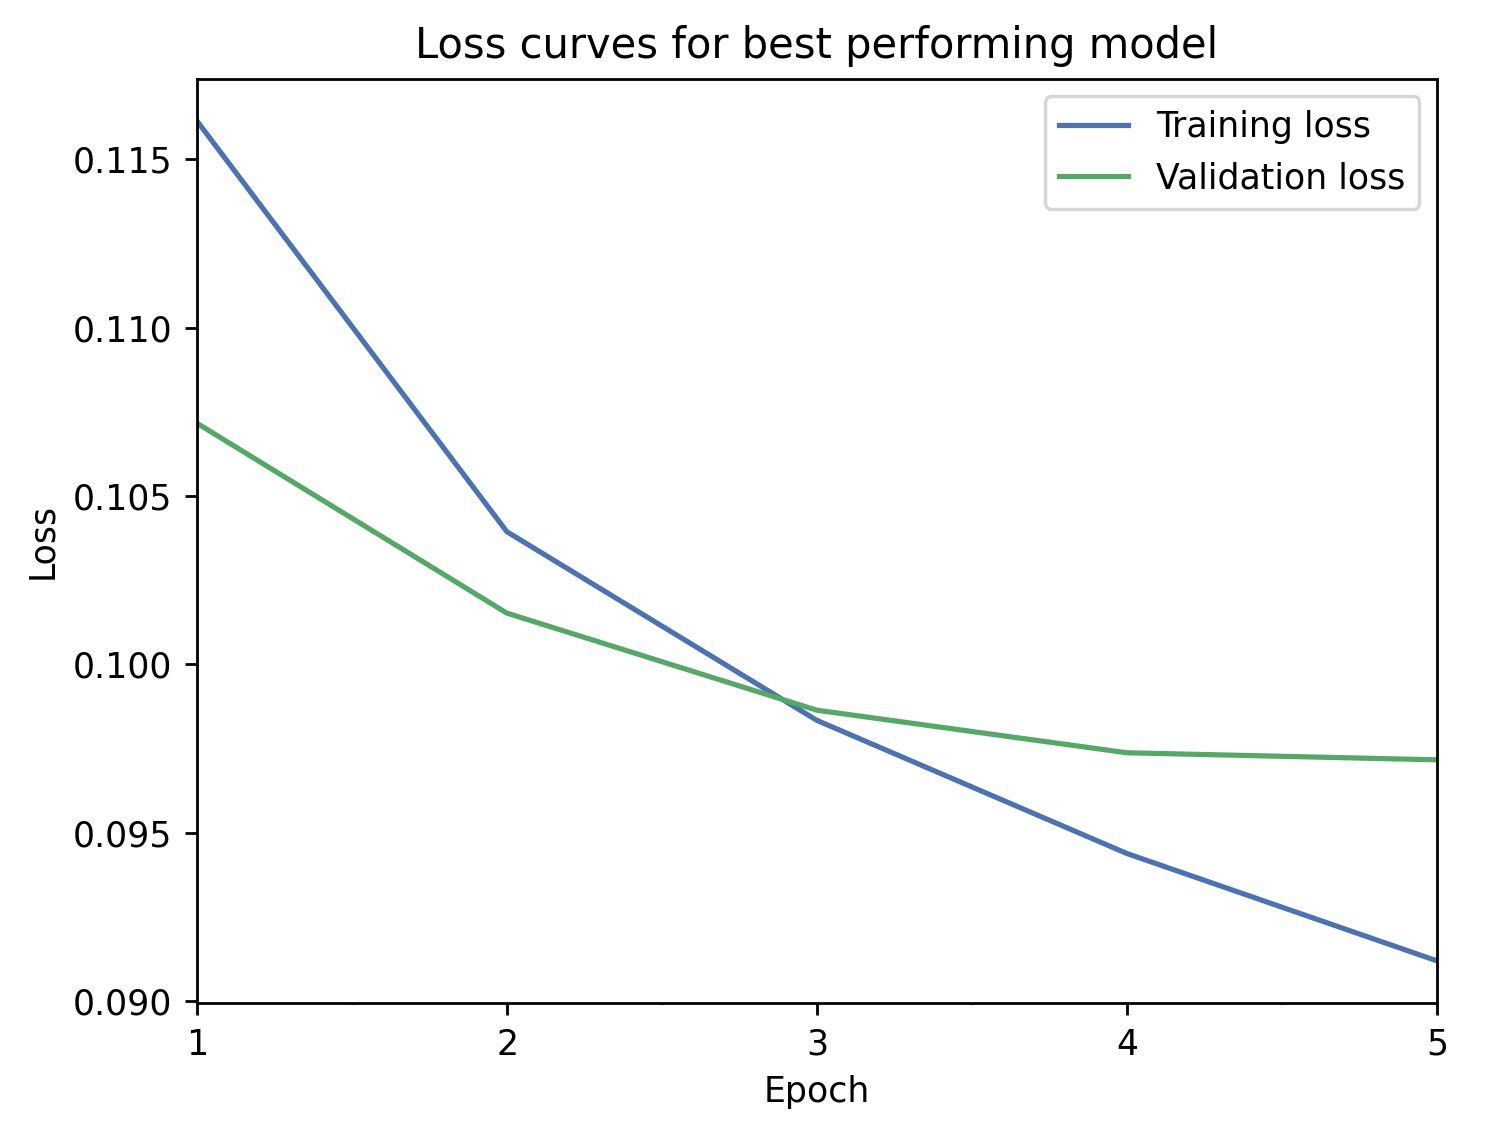
\includegraphics[width=0.5\textwidth]{project/img/loss_curves.png}
  \caption{Training and validation loss of the best performing model.}
  \label{lossCurves}
\end{figure}


\subsection{Conversion to Difficulty Prediction}\label{mlS23}

The architecture, as currently designed, only predicts puzzle themes. In early
experiments, multiple outputs and losses were attempted, but this led to
degradation of performance. To allow the model to predict puzzle difficulty, a
slight modification was made to the architecture (\Cref{mlS21}). 

The output 60 neurons were replaced with just 1: the difficulty rating
prediction. To make learning easier, all difficulties were scaled down by a
factor of 3500. As the difficulty rating range in the dataset is $(399, 3331)$
(\Cref{dataHistogram}), this scaled all ratings to a reasonable range. There
was no activation function for the final neuron.

The loss was changed to mean square error, and no other parameters were
changed. This model was trained with the same hyperparameters as the best
performing label prediction model (\Cref{mlS22}) for 5 epochs. This produced an
entirely new model.

\section{Visualisations of the Model}\label{mlS3}

Previously, the idea of chess pieces and squares interacting with each other
was shown (\Cref{chessPuzzleLinks}). With a trained model, this can now be
explored further. By extracting the attention values and weights from each of
the transformer layers, as the bitboards flow through the model, and unflattening
them back into a $8\times8$ chess board, some interesting patterns can be seen.

\subsection{Interpretation}

Attention values and weights are shown below for the puzzle which was used to
illustrate how transformers could work in this problem
(\Cref{chessPuzzleLinks}). The values diagram (\Cref{atnP}) shows each channel
of the chess board atthat stage in the model. In the case of this model, there
are 256 channels, each of size $8\times8$. 

The weights diagram (\Cref{atnP1}) shows the weights of the self-attention
within the transformer architecture. This diagram has 64 heatmaps, arranged in
a chess-like arrangement. Each heatmap represents the weights it assigns to the
other board locations when updating its own embedding. 

To see a concrete example, take the top left heatmap, corresponding to the
\texttt{a8} square. This value assigns a very positive weight to the
\texttt{g8} square (yellow dot in the top right), and a much lower (possibly
negative) weight to the middle ranks in the board.


\begin{figure}[H]
  \begin{minipage}{0.475\textwidth}
    \centering
    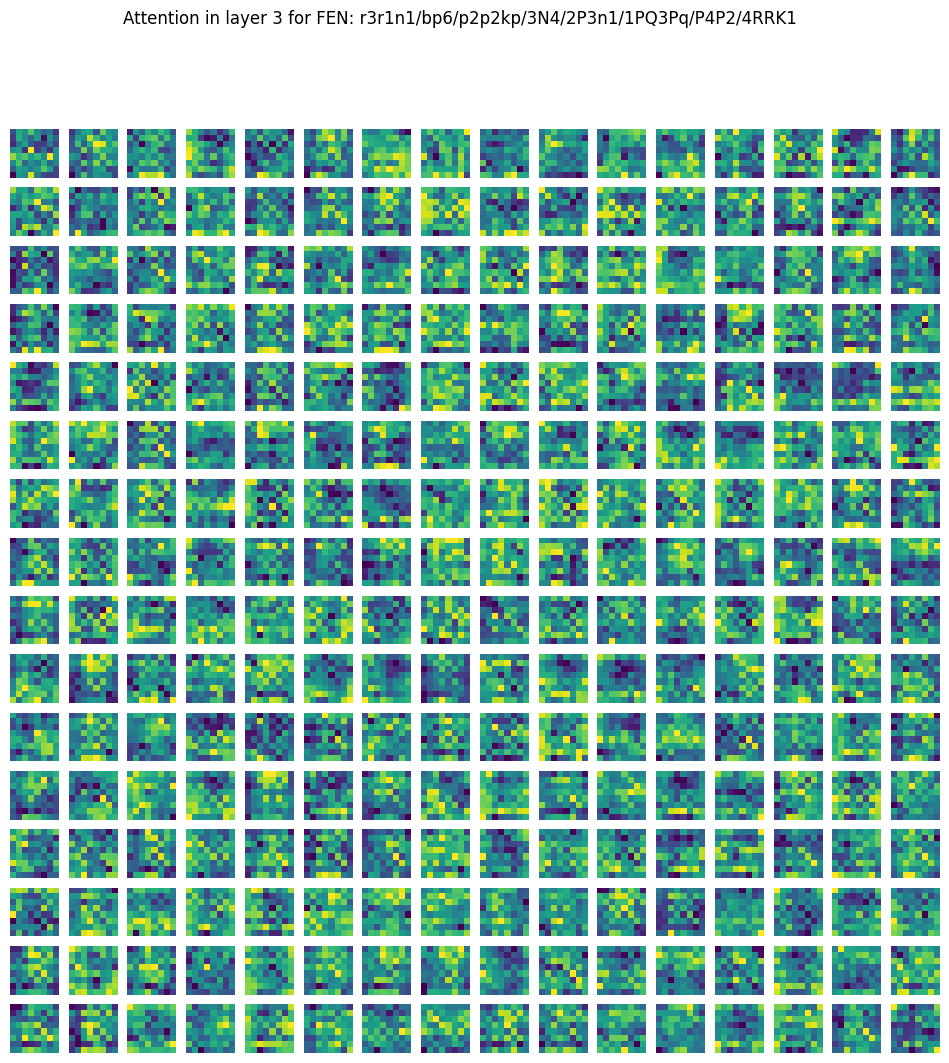
\includegraphics[width=\textwidth]{project/img/attention_maps/attention_3.png}
    \caption{Attention values in layer 3 of the transformer encoder.}
    \label{atnP}
  \end{minipage}
  \hspace{0.05\textwidth}
  \begin{minipage}{0.475\textwidth}
    \centering
    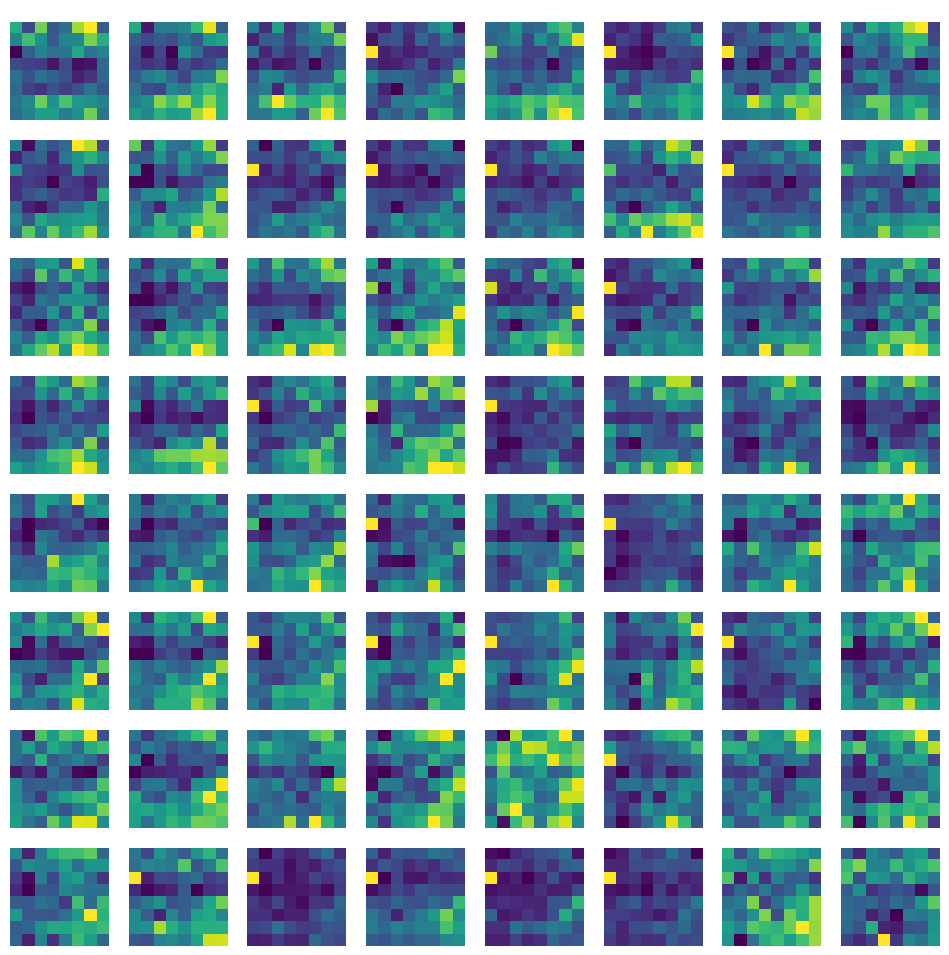
\includegraphics[width=\textwidth]{project/img/attention_maps/weights_4.png}
    \caption{Attention weights in layer 4 of the transformer encoder.}
    \label{atnP1}
  \end{minipage}
\end{figure}

\subsection{Attention Weights and Values of Single Chess Pieces}\label{mlS32}

In this section, a single chess piece is placed on \texttt{e4} and this
position is passed through the model. The corresponding attention value and
weight heatmaps are shown.

\paragraph{Rook} Horizontal and vertical patterns can be seen in both diagrams.
This, of course, stems from the moveset of the rook.

\begin{figure}[H]
  \begin{minipage}{0.475\textwidth}
    \centering
    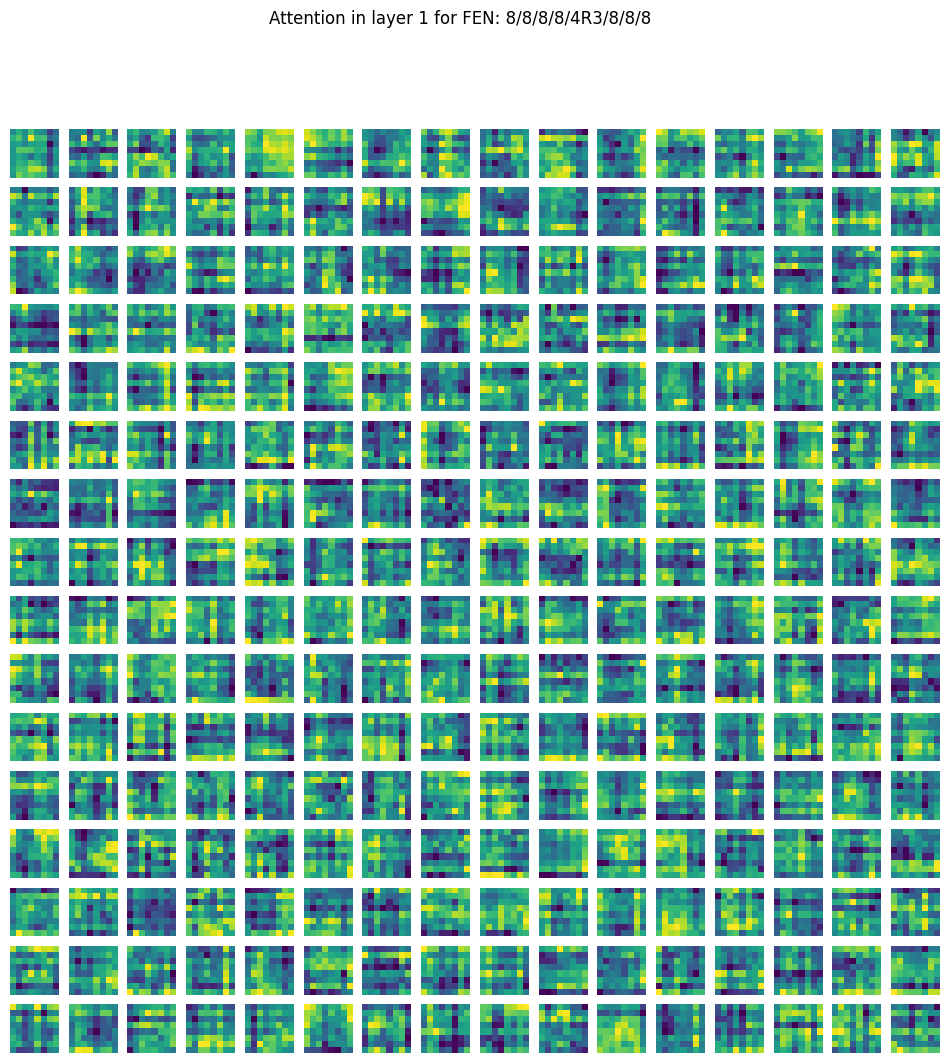
\includegraphics[width=\textwidth]{project/img/attention_maps/R_attention_1.png}
    \caption{Rook attention values.}
    \label{atnR1}
  \end{minipage}
  \hspace{0.05\textwidth}
  \begin{minipage}{0.475\textwidth}
    \centering
    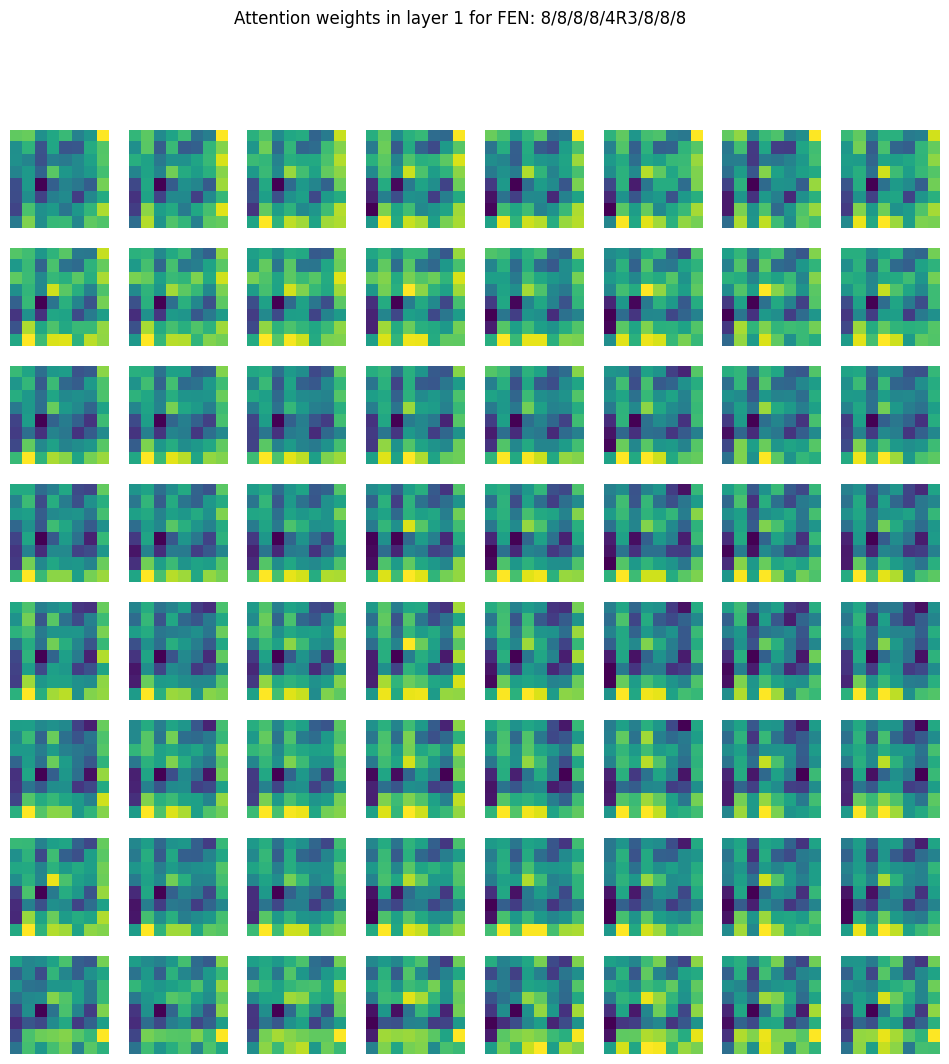
\includegraphics[width=\textwidth]{project/img/attention_maps/R_weights_1.png}
    \caption{Rook attention weights.}
    \label{atnR}
  \end{minipage}
\end{figure}

\paragraph{Bishop} This bishop is a light-squared bishop. Bishops can only move
diagonally, and this means that half of the board will never be accessible to
the bishop, which explains the checkerboard nature of the heatmaps.
Interestingly, the weights diagram (\Cref{atnB1}) shows how important the main
diagonal is, which is controlled by the bishop. Every other square takes it
into consideration when updating its own value.

\begin{figure}[H]
  \begin{minipage}{0.475\textwidth}
    \centering
    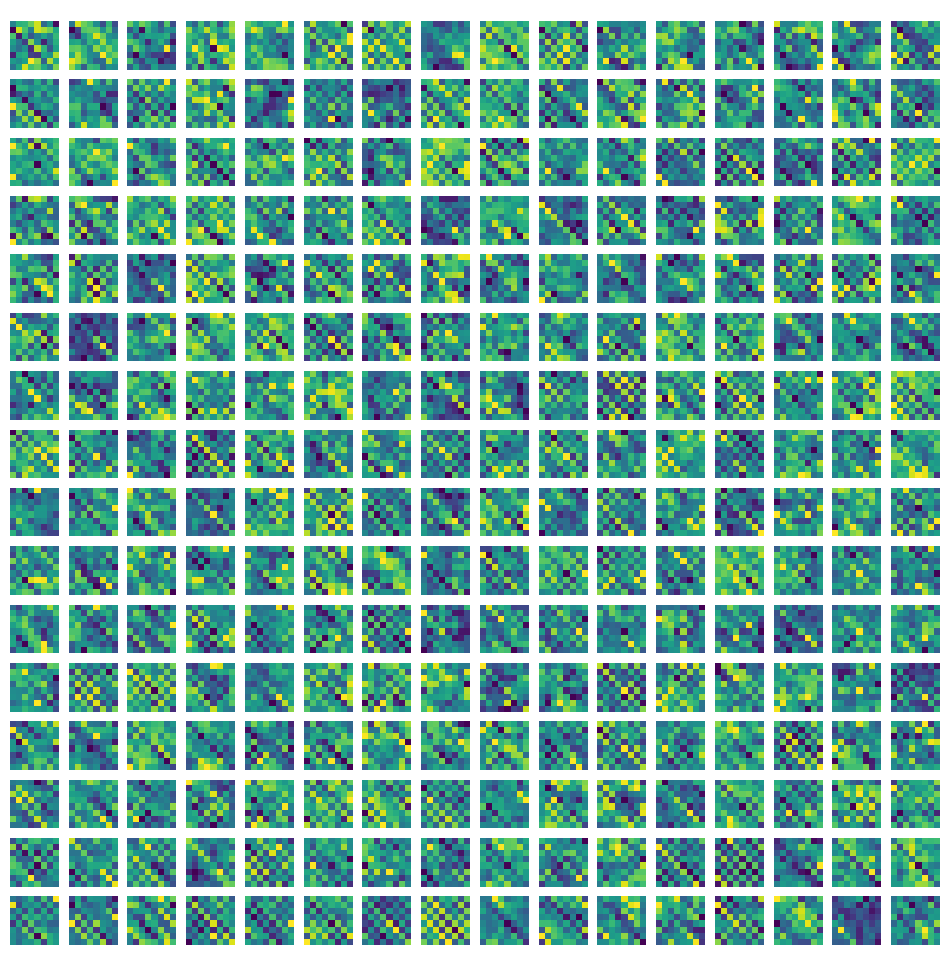
\includegraphics[width=\textwidth]{project/img/attention_maps/B_attention_4.png}
    \caption{Bishop attention values.}
    \label{atnB}
  \end{minipage}
  \hspace{0.05\textwidth}
  \begin{minipage}{0.475\textwidth}
    \centering
    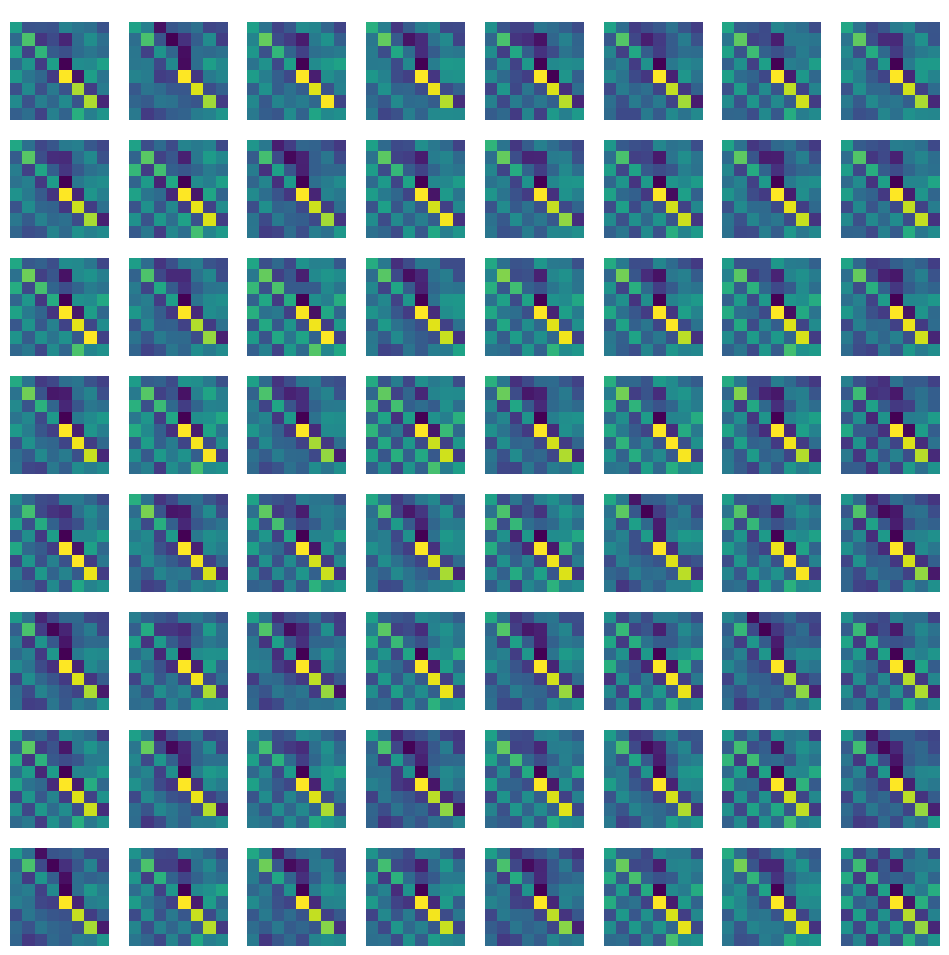
\includegraphics[width=\textwidth]{project/img/attention_maps/B_weights_4.png}
    \caption{Bishop attention weights.}
    \label{atnB1}
  \end{minipage}
\end{figure}

\paragraph{Queen} The queen combines the moveset of the rook and bishop, and
this can be seen in the heatmaps, as they are less structured. The weights
heatmap shows that the \texttt{h7} square is important -- this is possibly
because many checkmates are delivered by the queen on this square, and the
queen has vision of \texttt{h7} from \texttt{e4}.

\begin{figure}[H]
  \begin{minipage}{0.475\textwidth}
    \centering
    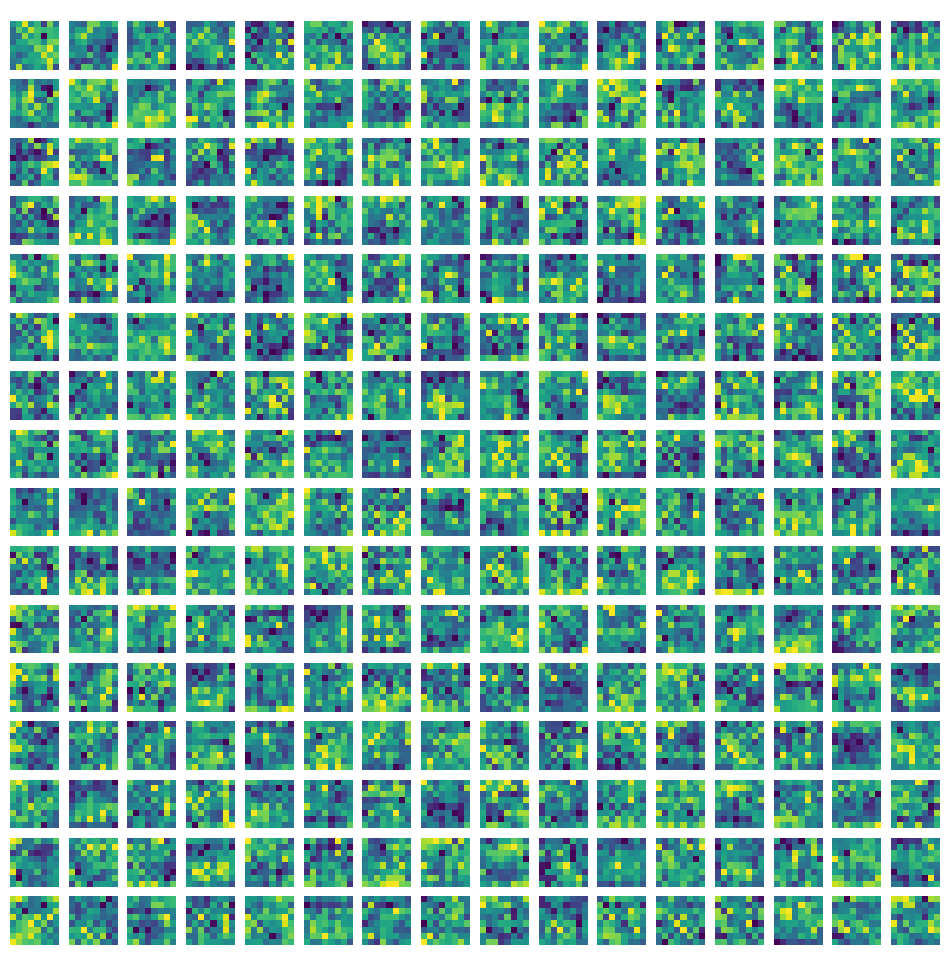
\includegraphics[width=\textwidth]{project/img/attention_maps/Q_attention_6.png}
    \caption{Queen attention values.}
    \label{atnQ}
  \end{minipage}
  \hspace{0.05\textwidth}
  \begin{minipage}{0.475\textwidth}
    \centering
    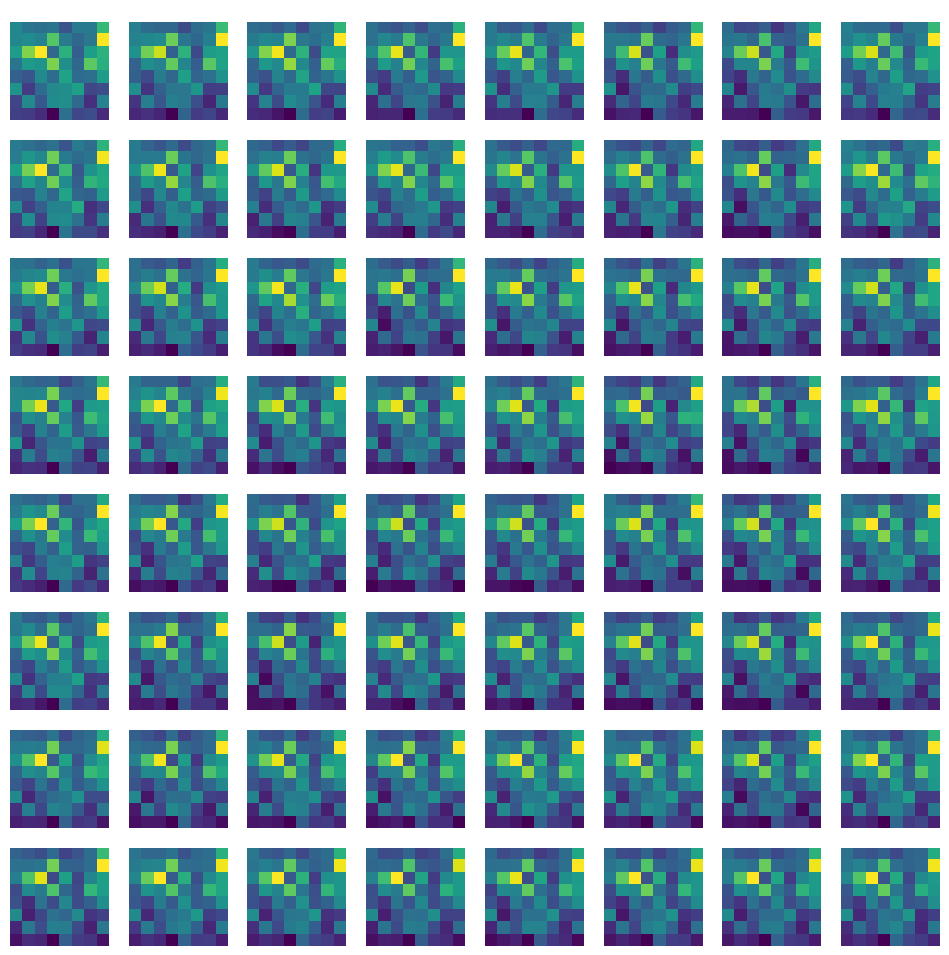
\includegraphics[width=\textwidth]{project/img/attention_maps/Q_weights_6.png}
    \caption{Queen attention weights.}
    \label{atnQ1}
  \end{minipage}
\end{figure}


\paragraph{Knight} The knight heatmaps have a checkerboard pattern similar to
the bishop's. This is likely a result of its moveset: a knight attacks
squares of the opposite colour to the square it is on.

\begin{figure}[H]
  \begin{minipage}{0.475\textwidth}
    \centering
    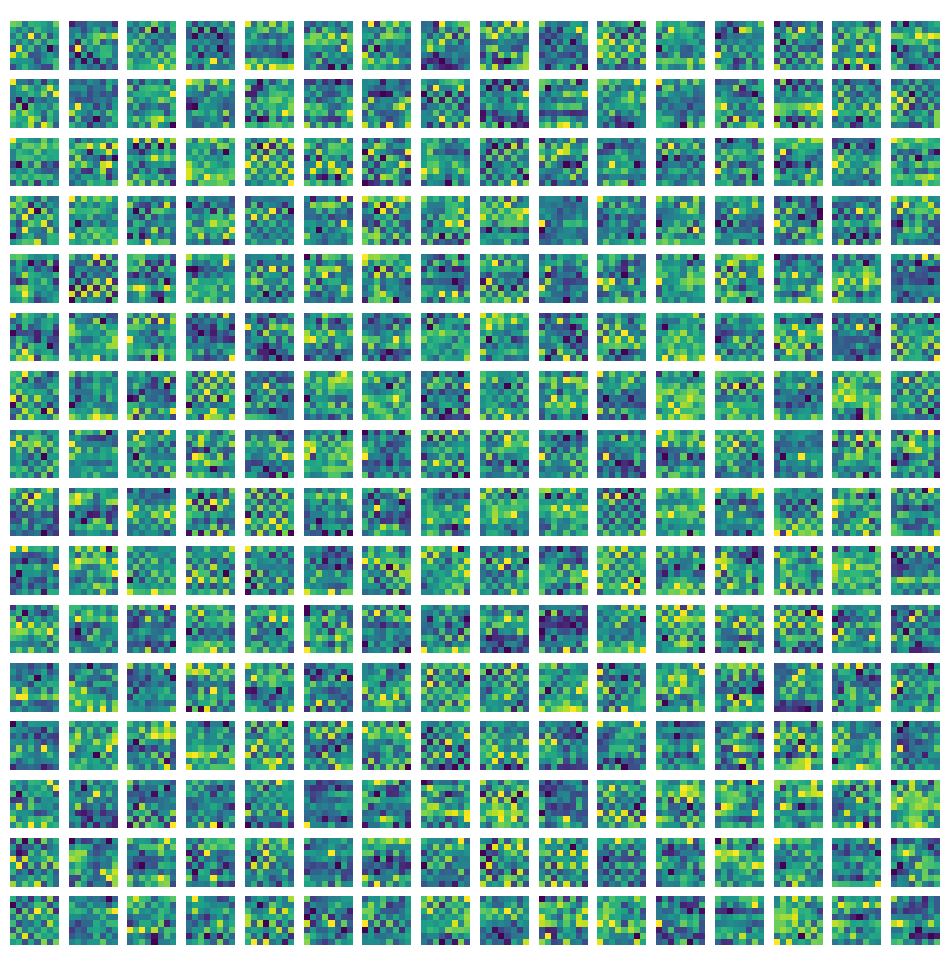
\includegraphics[width=\textwidth]{project/img/attention_maps/N_attention_1.png}
    \caption{Knight attention values.}
    \label{atnN}
  \end{minipage}
  \hspace{0.05\textwidth}
  \begin{minipage}{0.475\textwidth}
    \centering
    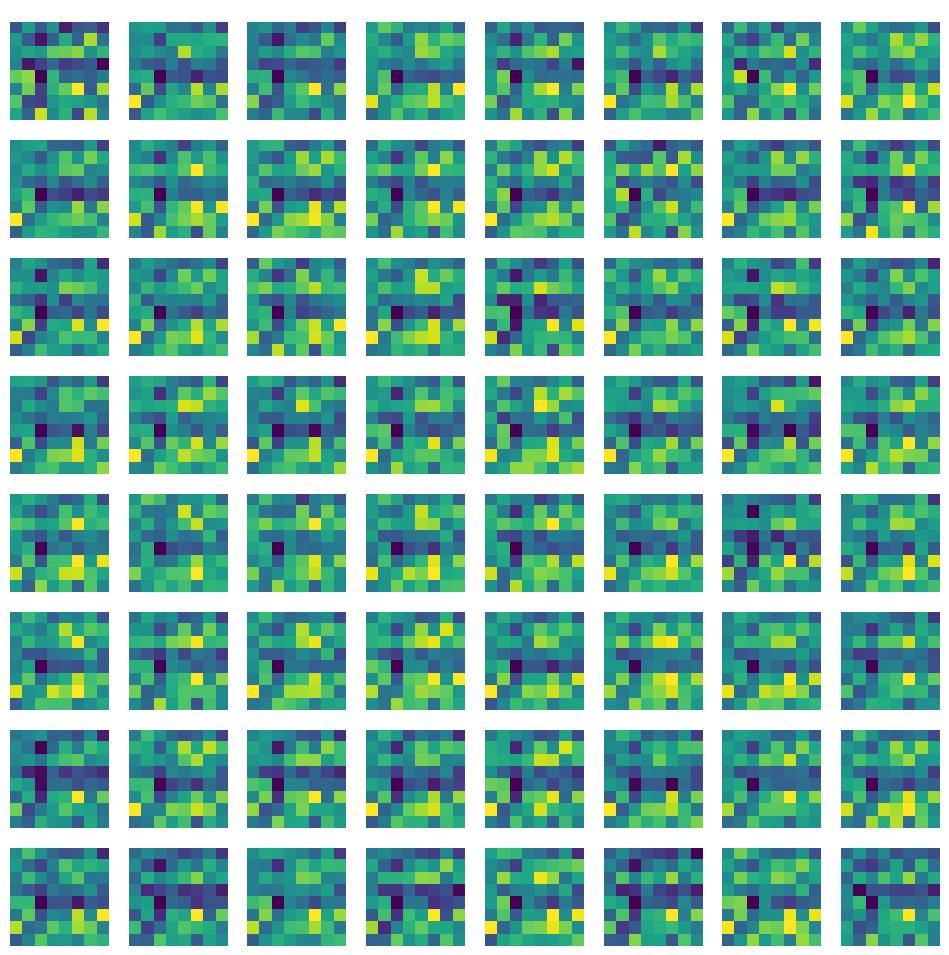
\includegraphics[width=\textwidth]{project/img/attention_maps/N_weights_1.png}
    \caption{Knight attention weights.}
    \label{atnN1}
  \end{minipage}
\end{figure}

\paragraph{Pawn} Pawns can only move forwards and usually come in groups,
aligned horizontally. This is clearly seen in both of the attention heatmaps.
The weights heatmap (\Cref{atnP1}) especially highlights this: the files in
front of the pawn and behind the pawn are important, as these usually have
pawns supported by, or supporting the \texttt{e4} pawn.

\begin{figure}[H]
  \begin{minipage}{0.475\textwidth}
    \centering
    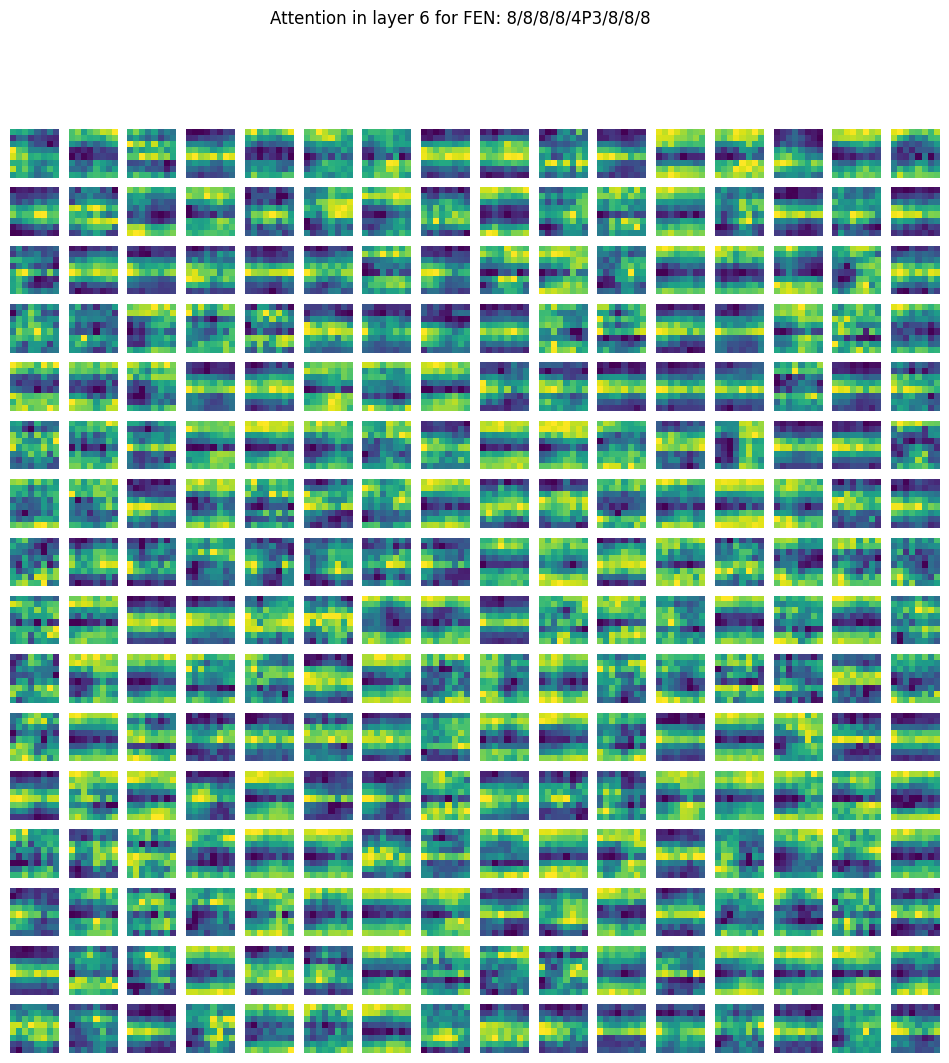
\includegraphics[width=\textwidth]{project/img/attention_maps/P_attention_6.png}
    \caption{Pawn attention values.}
    \label{atnP}
  \end{minipage}
  \hspace{0.05\textwidth}
  \begin{minipage}{0.475\textwidth}
    \centering
    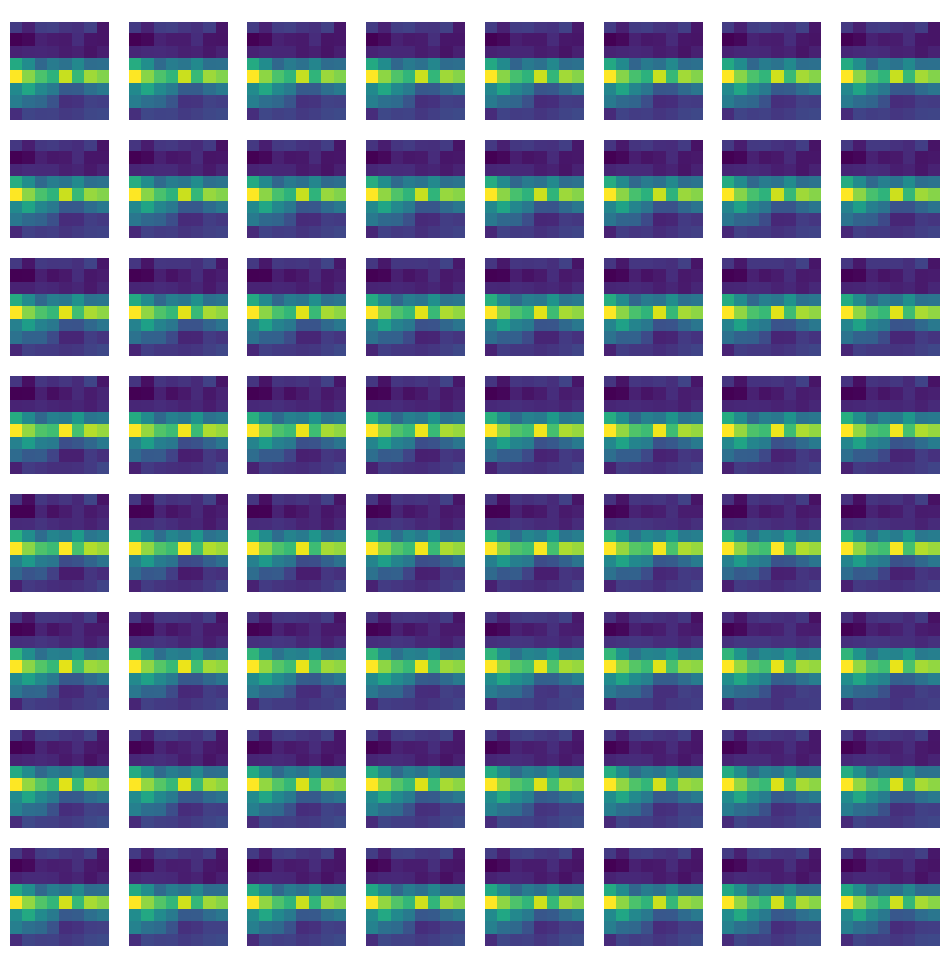
\includegraphics[width=\textwidth]{project/img/attention_maps/P_weights_6.png}
    \caption{Pawn attention weights.}
    \label{atnP1}
  \end{minipage}
\end{figure}


\paragraph{King} Finally, the king. The attention weights heatmap
(\Cref{atnK1}) shows heavy importance of the \nth{1} and \nth{8} files -- where
the kings are usually located.


\begin{figure}[H]
  \begin{minipage}{0.475\textwidth}
    \centering
    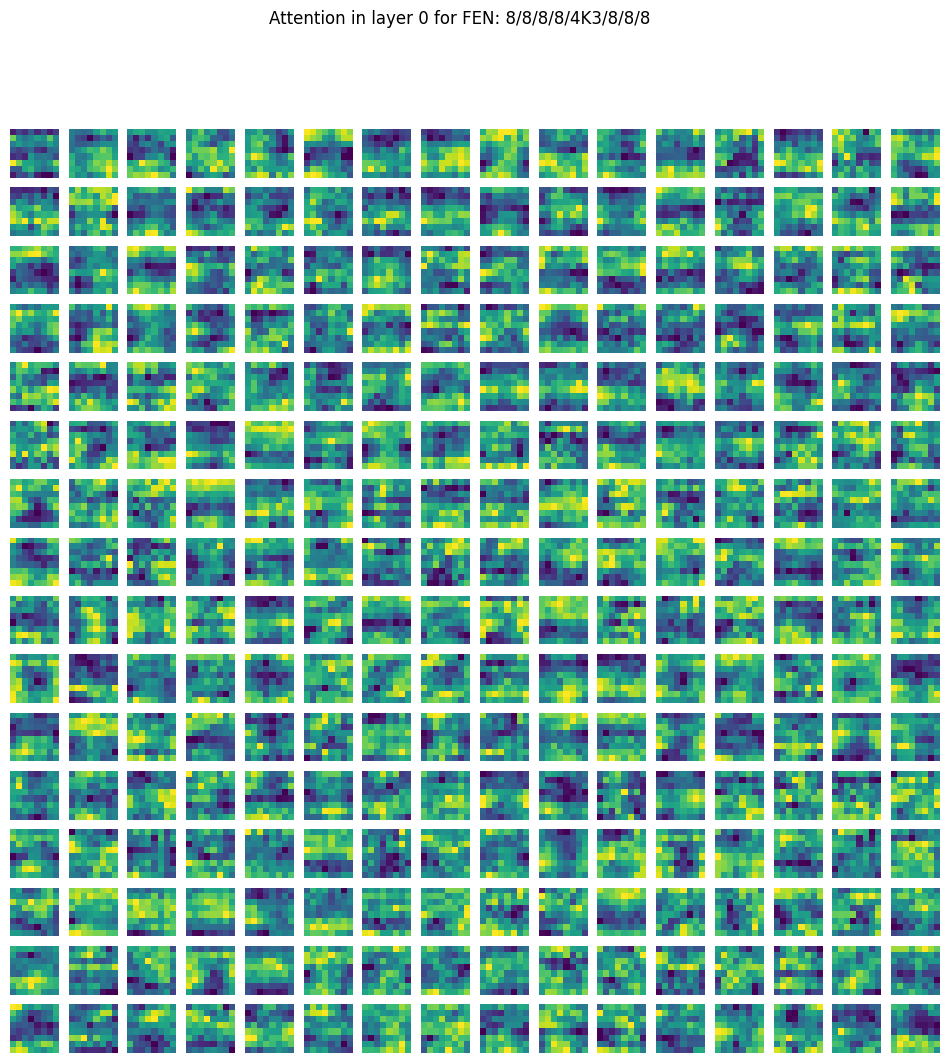
\includegraphics[width=\textwidth]{project/img/attention_maps/K_attention_0.png}
    \caption{King attention values.}
    \label{atnK}
  \end{minipage}
  \hspace{0.05\textwidth}
  \begin{minipage}{0.475\textwidth}
    \centering
    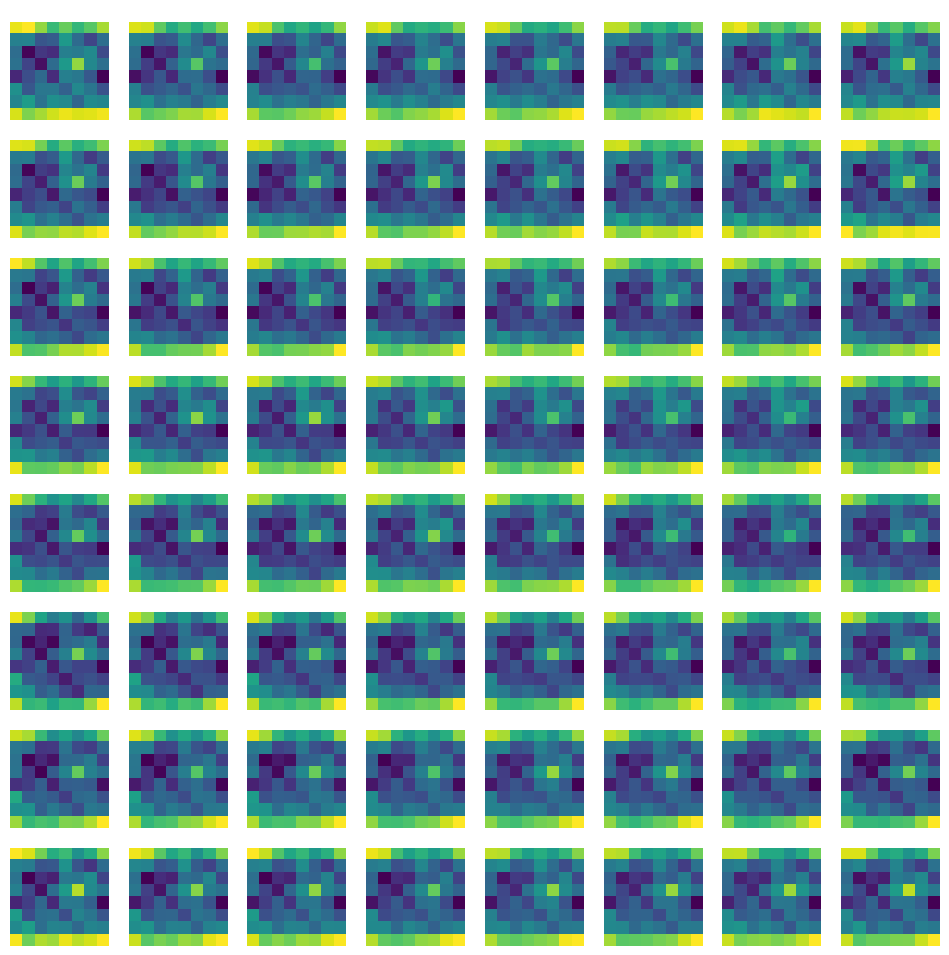
\includegraphics[width=\textwidth]{project/img/attention_maps/K_weights_0.png}
    \caption{King attention weights.}
    \label{atnK1}
  \end{minipage}
\end{figure}

\subsection{Discussion}\label{mlS33}

The patterns generated by the model (\Cref{mlS32}) are incredible, given the
model has 0 information about the game of chess other than a collection of
static positions and labels. This is reminiscent of the work of
\citet{chess2vec} (\Cref{bg4}), who were able to find success without
explicitly implementing chess logic.

This shows that transformers have untapped potential in the area of chess, as
these patterns were learned in order to label puzzles effectively. Playing
chess, which would require a deeper understanding of piece interactions and
positions, was not a target, and despite this, progress towards it seems to
have been made.




\chapter{The Tree-Based Approach}\label{treeChapter}

In this chapter, a different novel approach to puzzle classification is
proposed, focusing on the applications of a custom distance function defined
between chess puzzles' meaningful search trees.

Initially, the concept of labelled search trees and distance is introduced
(\Cref{treeS1}). This includes a high-level description of how to create these
trees (\Cref{treeS12,treeS13}) and how to measure distance between them
(\Cref{treeS21}).

Unsupervised clustering (\Cref{treeS2}) naturally follows these concepts. The
results of this are shown (\Cref{treeS22}), along with concrete examples and
visualisations (\Cref{treeS23}).

Afterwards, $k$-Nearest Neighbours (\Cref{treeS3}) is used for the downstream
task of puzzle label and difficulty rating prediction. Its performance is
evaluated and compared to the deep learning approach (\Cref{mlChapter}) in the
next chapter.

\section{Overview}\label{treeS1}

This method seeks to combine and build upon two approaches seen in the above
literature review: the tree-based puzzle difficulty classification by
\citet{chessTrees} and chess position similarity using dynamic features by
\citet{chessMotifs} (\Cref{typeAndDifficultyReview}).

By combining these approaches to construct meaningful search trees with
additional node labels, defining a distance function for individual chess
moves, and applying a labelled tree edit distance function
\citep{editDistTrees}, it will be possible to calculate `closeness' of chess
puzzles. 

\subsection{Representing Puzzles With Labelled Trees}\label{treeS11}

As explored by \citet{chessTrees}, `meaningful search trees' have predictive
possibility of a puzzle's difficulty. These trees are constructed by analysing
powerful moves that either gain, or at least do not worsen a side's position. 

By additionally labelling these trees with move information, this work can be
built upon. To demonstrate the intuition behind this idea, there are two
labelled search trees (\Cref{tree1,tree2}) of visually distinct, but tactically
similar chess positions (\Cref{chess5,chess6}), which were found by
\citet{chessLanguage} (\Cref{concWork}). 

In these trees, algebratic notation of the moves is shown, along with 4
slash-delimited integers, which correspond to: pieces attacked, pieces
defended, number of attackers, number of defenders.\footnote{As the moves must
be legal, this means a king move will never have any attackers, and any
check/mate will have at least 1 piece attacked: the enemy king.} While the 2
trees do not look similar visually (their size being the main problem), the
first 3 halfmoves are almost identical. 

\begin{figure}[H]
  \begin{minipage}{0.475\textwidth}
    \centering
    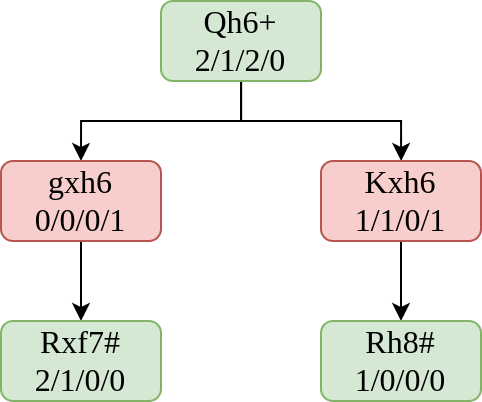
\includegraphics[width=\textwidth]{project/img/trees/1.drawio.png}
    \caption{Labelled search tree for game in \ref{chess5}}
    \label{tree1}
  \end{minipage}
  \hspace{0.05\textwidth}
  \begin{minipage}{0.475\textwidth}
    \centering
    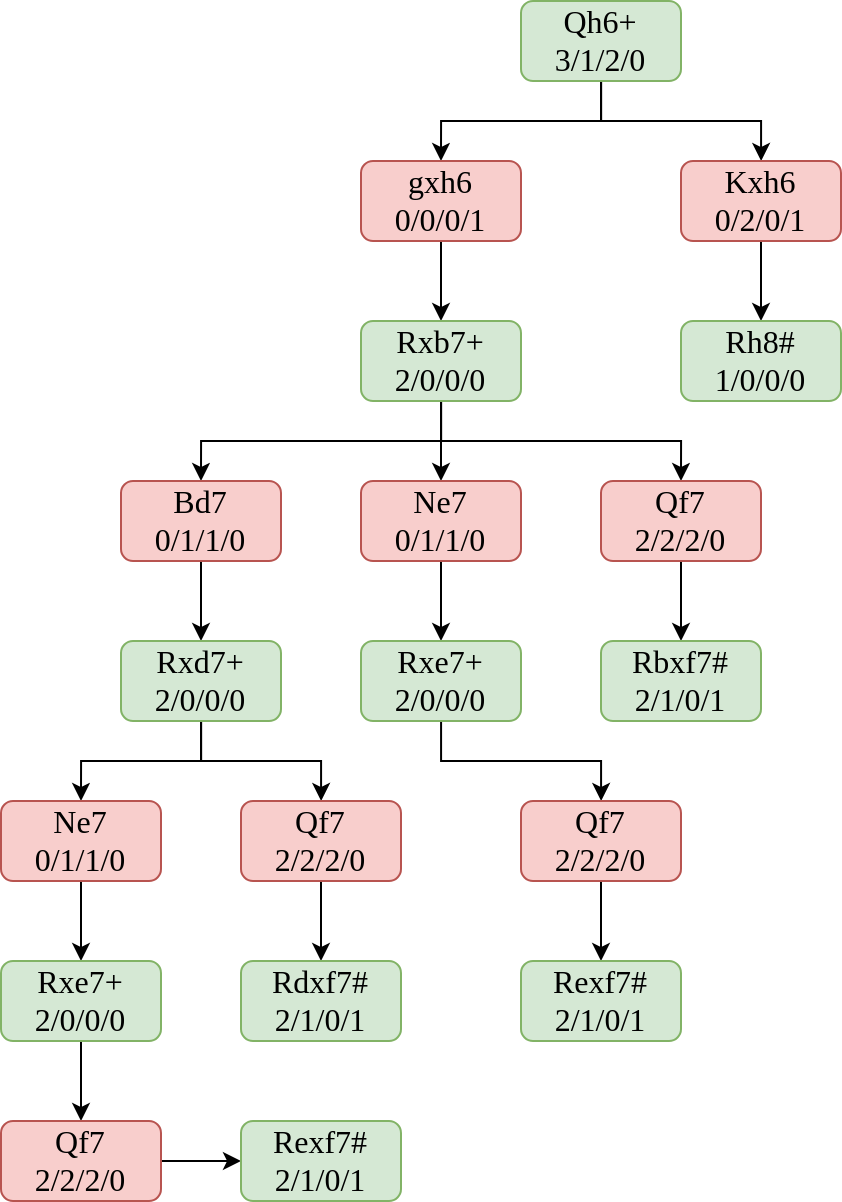
\includegraphics[width=\textwidth]{project/img/trees/2.drawio.png}
    \caption{Labelled search tree for game in \ref{chess6}}
    \label{tree2}
  \end{minipage}
\end{figure}

A clearer example of tree (\Cref{tree3,tree4}) similarity can be seen in
simpler puzzles (\Cref{puzzle5,puzzle6}). Both of these chess puzzles feature a
\emph{rook sacrifice}, and an imminent queen checkmate helped by the powerful
light-squared bishop. This similarity is not immediately obvious, but the
search trees for these puzzles is almost identical, except for minor
attacker/defender discrepancies. These puzzles were already successfully
grouped by \citet{chessMotifs}.

\begin{figure}[H]
  \begin{minipage}[t]{0.475\textwidth}
    \centering
    \chessboard[setfen= 4r1k1/1b3pp1/4p3/p2r4/7R/2B1Q1PP/P1P1RP1K/1q6 w - -
    0 1]
    \caption{Taken from `Automatic Recognition of Similar Chess Motifs' by
    \citet{chessMotifs}. White mates in three moves (\texttt{1.Rh8+ Kxh8 2.Qh6+
    Kg8 3.Qxg7#}).}
    \label{puzzle5}
  \end{minipage}
  \hspace{0.05\textwidth}
  \begin{minipage}[t]{0.475\textwidth}
    \centering
    \chessboard[setfen=r5k1/5pp1/8/3p3R/2q4P/PbB2P2/1P1Q2P1/K7 w q - 0 1]
    \caption{Also taken from `Automatic Recognition of Similar Chess Motifs' by
    \citet{chessMotifs}. White mates in three with the same moves as the puzzle
    on the left.}
    \label{puzzle6}
  \end{minipage}
\end{figure}

\begin{figure}[H]
  \begin{minipage}{0.475\textwidth}
    \centering
    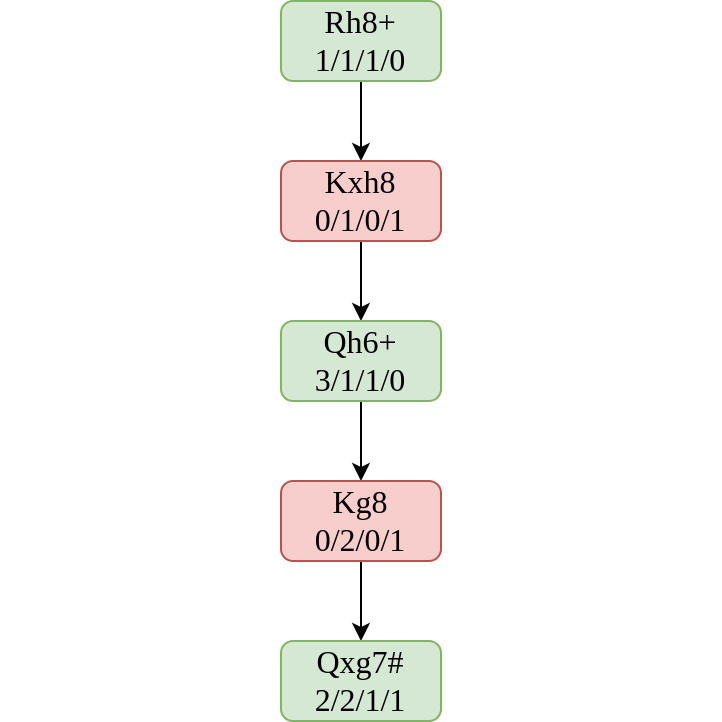
\includegraphics[width=\textwidth]{project/img/trees/3.drawio.png}
    \caption{Labelled search tree for the game above (\Cref{puzzle5}).}
    \label{tree3}
  \end{minipage}
  \hspace{0.05\textwidth}
  \begin{minipage}{0.475\textwidth}
    \centering
    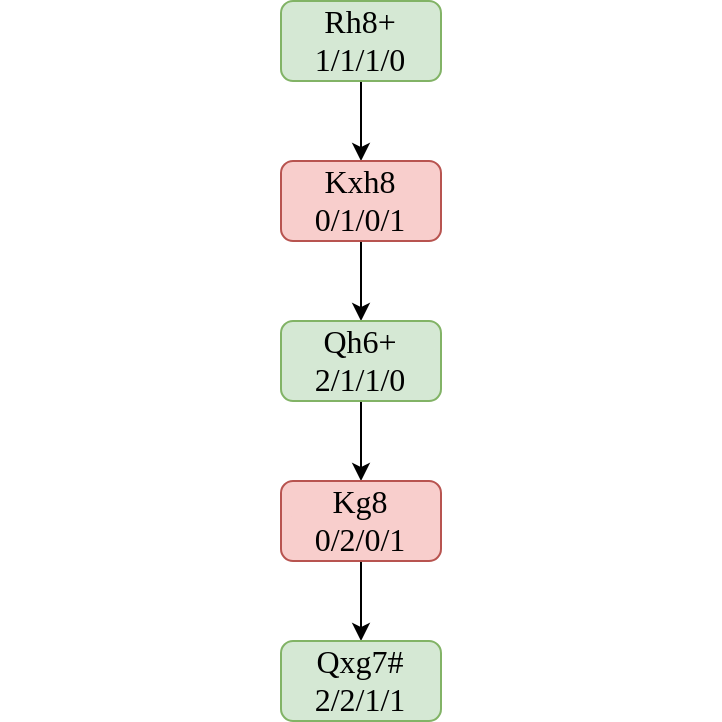
\includegraphics[width=\textwidth]{project/img/trees/4.drawio.png}
    \caption{Labelled search tree for the game above (\Cref{puzzle6}).}
    \label{tree4}
  \end{minipage}
\end{figure}

\subsection{Meaningful Tree Generation}\label{treeS12}

Similar to the work of \citet{chessTrees}, Stockfish (depth=20) was used to
generate meaningful trees of a maximum depth of 5 ply. Each level of the tree
has a maximum of 4 possible moves that are within 100 centipawns (arbitrarily
chosen) of the best move. To simplify analysis, all puzzles are transformed to
be from White's perspective.

\citet{chessTrees} writes: ``[A high branching factor] means that the position
is already so strong that it no longer matters what move the player chooses
because almost everything wins.''; the tree search is terminated if the best 4
moves for the losing side are within 100 centipawns. While this differs from
the quote above, it causes trees to terminate when the puzzle is completed (any
move for the losing side is equally bad), as opposed to one move before (any
move for the winning side is equally good). Finally, a checkmate naturally
indicates that the puzzle is solved. 

This analysis is continued until either every branch of the puzzle is
exhausted, whether because it has solved the puzzle, or ran out of the maximum
depth of 5.

Whilst generating the tree nodes, each move is annotated with a list of
attributes describing the properties of these move, such as the name of the
piece, whether it delivers check, and how many pieces it is defended by.

In total, 3.8 million game trees were generated, which took about 10000 hours
of CPU time. This was done with the help of the Department of Computing's
HTCondor cluster, managed by \citet{csgCondor}.

\subsection{What Makes Chess Moves Similar?}\label{treeS13}

To compare arbitrary tree nodes, a distance function was created -- this can be
used in the tree edit algorithm to find the distance between trees. The
properties of the moves in each node are compared, and any difference incurs a
penalty (\Cref{distanceTable}). These penalties are completely arbitrary and
were chosen by an intermediate chess player.

The penalty for adding or removing a node was set to 250. The final distance
between the node is given by the sum of all the individual penalties,
multiplied by a `depth multiplier'. These multipliers heavily discourage puzzle
difference at the beginning of the solution, and allow greater differences
towards the end. In early experiments, it was found that puzzles may have a
similar tactic at the beginning, which is crucial to their similarity, and a
different ending, which is less important. The depth multipliers are: $4, 1,
0.5, 0.25, 0.1, 0.05$ for depths $0$ through to $5$, respectively.

\begin{table}[H]
  \centering
  \begin{tabular}{lrl}
    Condition & Penalty & Note \\
    \hline
    Different colour & $\infty$ & Implementation detail \\
    &&\\
    Pieces are queen/rook & $25$ & Heavy pieces are used similarly \\
    Pieces are queen/bishop& $50$ & Both can attack diagonally \\
    Pieces are different and not QR/QB& $100$ & \\
    &&\\
    Differing source rank/file/diagonals & $3$ each & There are two diagonal
    directions:\\
    Differing target rank/file/diagonals & $3$ each & parallel to
    \texttt{a1}-\texttt{h8} and parallel to \texttt{a8}-\texttt{h1}. \\
    Chebyshev move distances $d_1, d_2$ & $|d_1-d_2|$ & Move distance is often
    not important \\
    &&\\
    Capture and non-capture & $50$ & \\
    Capture of different pieces & $10$ & \\
    Checking and non-checking & $25$ & \\
    Mate and non-mate & $50$ & \\
    &&\\
    Number of enemies attacked, $n_1, n_2$ & $3|n_1-n_2|$ & \\
    Number of allies defended, $n_1, n_2$ & $2|n_1-n_2|$ & \\
    Number of attackers, $n_1, n_2$ & $3|n_1-n_2|$ & \\
    Number of defenders, $n_1, n_2$ & $2|n_1-n_2|$ & \\
  \end{tabular}
  \caption{Breakdown of the node distance function for meaningful move trees}
  \label{distanceTable}
\end{table}

This distance function defines a distance between nodes of move trees. Together
with the unordered labelled tree edit distance algorithm by \citet{editDistTrees},
any two chess puzzles can now be compared. 

The initial results are shown in \Cref{distanceComparisons}, where 3 pairs of
similar puzzles are compared: a \emph{back-rank mate-in-one}
\Cref{chess1,chess2}), a \emph{rook sacrifice} featuring \emph{mate-in-three}
(\Cref{puzzle5,puzzle6}), and finally, a complex mating sequence with a
\emph{queen sacrifice} (\Cref{chess5,chess6}). 

Due to the design of the distance function, puzzles with the same meaningful
move tree have a distance of 0, naturally. However, as the nodes are labelled
with extra parameters, two puzzles with identical solutions do not necessarily
have a distance of 0.

It should also be noted that this distance function, while being symmetric,
does not satisfy the triangle inequality. Taking 3 nodes with identical
parameters except the piece and start square, say, \texttt{Qc4e4},
\texttt{Rc4e4}, \texttt{Bc2e4}, it is clear that $d(\texttt{Rc4e4},
\texttt{Bc2e4}) = 100 + 9 > 25 + (50 + 9) = d(\texttt{Rc4e4}, \texttt{Qc4e4}) +
d(\texttt{Qc4e4, Bc2e4})$.

These results show that this distance function can be used to compare puzzles
and detect if a pair is similar, as the distance between manually curated
similar puzzles is distinctly lower than the distance between non-similar
puzzles.

\begin{table}[H]
  \centering
  \begin{tabular}{r|cccccc}
    Figure &
    \ref{chess1}&\ref{chess2}&\ref{puzzle5}&\ref{puzzle6}&\ref{chess5}&\ref{chess6}
    \\
    \hline
    \ref{chess1} & $0$ & $232$ & $978.5$ & $982.5$ & $1422$ & $1714$ \\ 
    \ref{chess2} & $232$ & $0$ & $1086.5$ & $1082.5$ & $1278$ & $1586$ \\
    \ref{puzzle5} & $978.5$ & $1086.5$ & $0$ & $46.5$ & $789$ & $1033.15$ \\
    \ref{puzzle6} & $982.5$ & $1082.5$ & $46.5$ & $0$ & $795$ & $1035.15$ \\
    \ref{chess5} & $1422$ & $1278$ & $789$ & $795$ & $0$ & $417$ \\
    \ref{chess6} & $1714$ & $1586$ & $1033.15$ & $1035.15$ & $417$ & $0$ \\
  \end{tabular}
  \caption{Distance matrix for a selection of chess puzzles.}
  \label{distanceComparisons}
\end{table}

\subsection{Finding Similar Positions Given a Puzzle}\label{treeS21}

Unfortunately, generating a larger distance matrix is prohibitively expensive,
as it scales quadratically with the number of positions -- calculating this for
the whole Lichess database is difficult. By extracting just one row, however,
which scales linearly, a set of puzzles can be ranked by similarity to a given
puzzle.

For a simple \emph{back-rank mate-in-one} puzzle, this is incredibly effective.
With the basic puzzle (\Cref{chess1}), similar positions (\Cref{m11,m22}) can
be found in the Lichess puzzle databse. These positions are arguably more
complex as there are more pieces on the board, making it harder to find the
winning move, but nonetheless feature a \emph{back-rank mate-in-one}.

With a more complex position, such as the complex \emph{mate-in-two}
(\Cref{chess5}), positions in Figures \ref{mag1} and \ref{mag2} are returned.
These do not feature exactly the same tactic, but they are nonetheless similar,
featuring a \emph{rook sacrifice} on \texttt{h3} and different mates depending
on White's response.

\begin{figure}[H]
  \begin{minipage}[t]{0.475\textwidth}
    \centering
    \chessboard[setfen= 6k1/pr4pR/2p2pP1/2Pp4/5N2/P1r2P2/3RP3/3K4 b - - 1
    28]
    \caption{Distance $40$ to Figure \ref{chess1}. Solution:
    \texttt{1...Rb1\#}}
    \label{m11}
  \end{minipage}
  \hspace{0.05\textwidth}
  \begin{minipage}[t]{0.475\textwidth}
    \centering
    \chessboard[setfen=1r4k1/6p1/p1R1p2p/8/P6P/3R4/2P2rP1/3K4 b - - 0 30]
    \caption{Distance $0$ to Figure \ref{chess1}. Solution:
    \texttt{1...Rb1\#}}
    \label{m22}
  \end{minipage}
\end{figure}

\begin{figure}[H]
  \begin{minipage}[t]{0.475\textwidth}
    \centering
    \chessboard[setfen=2k3r1/p1p4p/8/pP1QR3/P2P3P/2P3r1/5RPK/3q4 b - - 2 30]
    \caption{Distance $255$ to Figure \ref{chess5}. Solution:
    \texttt{1...Rh3+ (2.Kxh3 Qh1\#) (2.gxh3 Qg1\#)}}
    \label{mag1}
  \end{minipage}
  \hspace{0.05\textwidth}
  \begin{minipage}[t]{0.475\textwidth}
    \centering
    \chessboard[setfen=6rk/pR6/2p4p/8/4PP2/P2P2r1/P2Q1RPK/q7 b - - 4 35]
    \caption{Distance $259$ to Figure \ref{chess5}. Solution identical to
    puzzle on the left.}
    \label{mag2}
  \end{minipage}
\end{figure}

\pagebreak

\section{Clustering}\label{treeS2}

\subsection{Unsupervised Clustering on Puzzle Distances}\label{treeS22}

To take this further, a distance matrix was constructed for a random sample of
20,000 puzzles from the Lichess puzzle database. A few labelled puzzles were
added to help with analysis of the results. A selection of unsupervised
clustering algorithms identify clusters of similar puzzles were ran. There is
no obvious vector space of search trees, which ruled out common algorithms like
K-means \citep{lloyd1982least}, Mean Shift \citep{fukunaga1975estimation}, and
others.

The attempted clustering algorithms were Agglomerative Clustering (average,
single, complete) \citep{szekely2005hierarchical}, DBSCAN \citep{dbscan}, and
HDBSCAN \citep{hdbscan} on this subset of the database. The results are shown
in \Cref{tabAC,tabDBSCAN,tabHDBSCAN}. Visualisations of the highlighted rows
can be seen in \Cref{treeS23}.

Parameters of the algorithms were varied, and since there is no obvious way to
analyse performance, some heuristics were recorded, such as number of clusters,
cluster size quartlies, and whether some simple puzzles
(\Cref{chess11,chess12,chess13,chess14}) were assigned to a cluster. A method
that has unusual cluster sizes, or one that fails to allocate even simple
puzzles to clusters is unlikely to be effective.

\begin{figure}[H]
  \begin{minipage}[t]{0.475\textwidth}
    \centering
    \chessboard[setfen=6k1/5ppp/8/8/8/8/r4PPP/1R4K1 w - - 0 1]
    \caption{\emph{Back-rank mate-in one}: \texttt{1.Rb8\#}}
    \label{chess11}
  \end{minipage}
  \hspace{0.05\textwidth}
  \begin{minipage}[t]{0.475\textwidth}
    \centering
    \chessboard[setfen=8/1N6/1K6/4k1p1/2P1Pp1p/4n2P/3R2P1/8 b - - 0 49]
    \caption{\emph{Knight fork}s with \texttt{1...Nxc4+}}
    \label{chess12}
  \end{minipage}
\end{figure}


\begin{figure}[H]
  \begin{minipage}[t]{0.475\textwidth}
    \centering
    \chessboard[setfen=
    r1bq1rk1/pp2nppp/1bn1p3/1N1pP3/1P6/P2B1N2/2P2PPP/R1BQK2R w KQ - 3 11]
    \caption{\emph{Greek gift sacrifice}: \texttt{1.Bxh7+ Kxh7 2.Ng5+}}
    \label{chess13}
  \end{minipage}
  \hspace{0.05\textwidth}
  \begin{minipage}[t]{0.475\textwidth}
    \centering
    \chessboard[setfen= 4r1k1/1b3pp1/4p3/p2r4/7R/2B1Q1PP/P1P1RP1K/1q6 w - -
    0 1]
    \caption{\emph{Mate-in-three} after a \emph{rook sacrifice}: \texttt{1.Rh8+ Kxh8 2.Qh6+
    Kg8 3.Qxg7\#}}
    \label{chess14}
  \end{minipage}
\end{figure}

\pagebreak

\begin{table}[H]
  \centering
  \begin{adjustbox}{width=0.9\textwidth}
    \begin{tabular}{lr|rccccrrrrrrr}
      \multicolumn{2}{l}{Parameters}&&\multicolumn{4}{c}{Puzzle is in a cluster}
      &&
      \multicolumn{6}{c}{Cluster size statistics} \\

      Linkage&Distance threshold&Number of clusters&\rotatebox{90}{Backrank M1} &
      \rotatebox{90}{Knight fork} & \rotatebox{90}{Greek gift} &
      \rotatebox{90}{Rook sac M3} & Outlier \% & \rotatebox{90}{Mean} &
      \rotatebox{90}{Min} & \rotatebox{90}{Q1} & \rotatebox{90}{Median} &
      \rotatebox{90}{Q3} & \rotatebox{90}{Max} \\

      \hline
      average&100&17040&Y&Y&Y&Y&0.0&1.17&1&1&1&1&178\\
      average&250&13812&Y&Y&Y&Y&0.0&1.45&1&1&1&1&1000\\
      average&500&8600&Y&Y&Y&Y&0.0&2.33&1&1&1&1&1863\\
      average&750&2759&Y&Y&Y&Y&0.0&7.25&1&1&1&2&2879\\
      average&1000&687&Y&Y&Y&Y&0.0&29.12&1&1&2&4&4069\\
      complete&100&17263&Y&Y&Y&Y&0.0&1.16&1&1&1&1&85\\
      complete&250&14064&Y&Y&Y&Y&0.0&1.42&1&1&1&1&611\\
      complete&500&9197&Y&Y&Y&Y&0.0&2.18&1&1&1&1&1000\\
      complete&750&3826&Y&Y&Y&Y&0.0&5.23&1&1&1&4&1780\\
      complete&1000&1404&Y&Y&Y&Y&0.0&14.25&1&2&3&8&2039\\
      single&100&16809&Y&Y&Y&Y&0.0&1.19&1&1&1&1&611\\
      single&250&13513&Y&Y&Y&Y&0.0&1.48&1&1&1&1&2642\\
      \rowcolor{lightgray} single&500&7418&Y&Y&Y&Y&0.0&2.7&1&1&1&1&9888\\
      single&750&1743&Y&Y&Y&Y&0.0&11.48&1&1&1&1&16224\\
      single&1000&231&Y&Y&Y&Y&0.0&86.6&1&1&1&1&19774\\


    \end{tabular}
  \end{adjustbox}
  \caption{Results of Agglomerative Clustering}
  \label{tabAC}
\end{table}

\begin{table}[H]
  \centering
  \begin{adjustbox}{width=0.9\textwidth}
    \begin{tabular}{rr|rccccrrrrrrr}
      \multicolumn{2}{l}{Parameters}&&\multicolumn{4}{c}{Puzzle is in a cluster}
      &&
      \multicolumn{6}{c}{Cluster size statistics} \\

      Epsilon&Minimum samples&Number of clusters&\rotatebox{90}{Backrank M1} &
      \rotatebox{90}{Knight fork} & \rotatebox{90}{Greek gift} &
      \rotatebox{90}{Rook sac M3} & Outlier \% & \rotatebox{90}{Mean} &
      \rotatebox{90}{Min} & \rotatebox{90}{Q1} & \rotatebox{90}{Median} &
      \rotatebox{90}{Q3} & \rotatebox{90}{Max} \\

      \hline
      50&3&45&&&&&93.28&29.82&7&9&13&28&365\\
      50&5&45&&&&&93.28&29.82&7&9&13&28&365\\
      50&7&45&&&&&93.28&29.82&7&9&13&28&365\\
      50&9&37&&&&&93.65&34.32&9&10&16&28&365\\
      100&3&43&Y&&&Y&83.69&75.86&7&11&21&41&1000\\
      100&5&43&Y&&&Y&83.69&75.86&7&11&21&41&1000\\
      100&7&43&Y&&&Y&83.69&75.86&7&11&21&41&1000\\
      100&9&38&Y&&&Y&83.88&84.84&9&13&26&51&1000\\
      250&3&36&Y&&Y&Y&67.36&181.39&7&9&25&87&2643\\
      250&5&36&Y&&Y&Y&67.36&181.39&7&9&25&87&2643\\
      250&7&36&Y&&Y&Y&67.36&181.39&7&9&25&87&2643\\
      250&9&32&Y&&Y&Y&67.60&202.56&9&13&30&112&2643\\
      500&3&5&Y&Y&Y&Y&37.03&2519.4&17&256&391&2039&9894\\
      500&5&5&Y&Y&Y&Y&37.03&2519.4&17&256&391&2039&9894\\
      \rowcolor{lightgray} 500&7&5&Y&Y&Y&Y&37.03&2519.4&17&256&391&2039&9894\\
      500&9&5&Y&Y&Y&Y&37.03&2519.4&17&256&391&2039&9894\\
      750&3&2&Y&Y&Y&Y&8.69&9133.0&2039&5586&9133&12680&16227\\
      750&5&2&Y&Y&Y&Y&8.69&9133.0&2039&5586&9133&12680&16227\\
      750&7&2&Y&Y&Y&Y&8.69&9133.0&2039&5586&9133&12680&16227\\
      750&9&2&Y&Y&Y&Y&8.69&9133.0&2039&5586&9133&12680&16227& \\

    \end{tabular}
  \end{adjustbox}
  \caption{Results of DBSCAN}
  \label{tabDBSCAN}
\end{table}

\begin{table}[H]
  \centering
  \begin{adjustbox}{width=0.9\textwidth}
    \begin{tabular}{rr|rccccrrrrrrr}
      \multicolumn{2}{l}{Parameters}&&\multicolumn{4}{c}{Puzzle is in a cluster}
      &&
      \multicolumn{6}{c}{Cluster size statistics} \\

      Cluster selection $\epsilon$&Min cluster size&Number of
      clusters&\rotatebox{90}{Backrank M1} &
      \rotatebox{90}{Knight fork} & \rotatebox{90}{Greek gift} &
      \rotatebox{90}{Rook sac M3} & Outlier \% & \rotatebox{90}{Mean} &
      \rotatebox{90}{Min} & \rotatebox{90}{Q1} & \rotatebox{90}{Median} &
      \rotatebox{90}{Q3} & \rotatebox{90}{Max} \\

      \hline

      0&3&1347&Y&Y&&Y&42.57&8.53&3&3&5&9&338\\
      0&5&801&Y&Y&&Y&49.21&12.69&5&6&8&12&347\\
      0&7&546&Y&Y&&Y&52.17&17.52&7&8&10&15&917\\
      0&9&342&&Y&Y&Y&59.84&23.49&9&11&14&19&386\\
      25&3&1156&&Y&Y&Y&44.91&9.53&3&4&5&10&355\\
      25&5&693&Y&Y&Y&Y&49.6&14.55&5&6&8&13&352\\
      25&7&462&Y&Y&Y&Y&53.16&20.27&7&8&11&16&980\\
      25&9&354&&Y&Y&Y&58.77&23.3&9&10&13&20&383\\
      50&3&1212&&Y&Y&Y&42.80&9.44&3&3&5&9&353\\
      50&5&706&&Y&Y&Y&48.61&14.56&5&6&8&12&384\\
      50&7&479&Y&Y&Y&Y&50.94&20.48&7&8&10&15&901\\
      50&9&330&Y&Y&Y&Y&59.0&24.85&9&10&13&20&379\\
      100&3&1123&Y&Y&Y&Y&41.14&10.49&3&3&5&8&1000\\
      100&5&624&Y&Y&Y&Y&46.9&17.02&5&6&8&11&1000\\
      \rowcolor{lightgray}100&7&410&Y&Y&Y&Y&51.72&23.55&7&8&10&15&1000\\
      100&9&276&Y&Y&Y&Y&55.06&32.57&9&10&13&19&1000\\
      250&3&928&Y&Y&Y&Y&33.90&14.25&3&3&5&8&2606\\
      250&5&541&Y&Y&Y&Y&37.46&23.13&5&6&8&11&2853\\
      250&7&355&Y&Y&Y&Y&41.18&33.15&7&8&9&14&2853\\
      250&9&226&Y&Y&Y&Y&43.72&49.82&9&10&12&17&2611\\


    \end{tabular}
  \end{adjustbox}
  \caption{Results of HDBSCAN}
  \label{tabHDBSCAN}
\end{table}

With these results, it is easy to identify the methods that really struggle to
create meaningful clusters out of the given chess puzzles. Namely, all variants
of Agglomerative Clustering produced results with either too many clusters
(10000+) of 1 puzzle each, or a megacluster consisting almost of the entire
subset of the database. It is not obvious what an appropriate cluster count is;
the Lichess database has 60 unique themes, which gives a very rough target.
However, these themes are not mutually exclusive, unlike the cluster membership
produced by these algorithms. 

The cluster membership of puzzles allowed some parameter combinations of DBSCAN
to be disqualified, specifically the lower epsilon ones. Epsilon is the
distance at which points are considered to be in one neighbourhood
\citep{dbscan}, and setting this too low means similar puzzles are not given
the same cluster. The small distance matrix (\Cref{distanceComparisons}) seen
above shows that manually selected similar puzzles can have a distance of 417,
and this is by no means an upper limit.

Another interesting result is the percentage of outliers -- puzzles which have
so little neighbours around them that they are not given a cluster and
considered noise. This number hovers at around 50\% for HDBSCAN
(\Cref{tabHDBSCAN}), and drops to about 8-9\% for DBSCAN (\Cref{tabDBSCAN}).
Unfortunately, the lowest percentage happens when DBSCAN identifies 2 clusters,
which is far too few to draw meaningful conclusions from.

\subsection{Visualisations of Puzzle Clusters}\label{treeS23}

To illustrate what these clusters look like, t-distributed Stochastic Neighbor
Embedding (t-SNE) was used, a method to visualise high dimensional data in two
or three dimensions, developed by \citet{tsne}. It should be noted that these
visualisations can be quite misleading \citep{wattenberg2016how}, but they are
nonetheless helpful for developing some sense of the structure and clustering.

In the following diagrams, vibrant points denote the clusters of the puzzles
above. Faintly coloured crosses are clusters which do not contain any of those
puzzles. Faintly coloured black points are outliers. The legend contains only
the clusters of the known puzzles, as there is no obvious label to the other
generated clusters.

\Cref{tsne1} shows a t-SNE visualisation of the low-performing Agglomerative
Clustering. There are no outliers in this method, and every puzzle is part of a
cluster, causing multicoloured blobs. The biggest cluster, containing just over
half of the puzzles, is the cyan one, spanning multiple t-SNE blobs. This
megacluster contains all but one of the puzzles, the \emph{back-rank
mate-in-one} (\Cref{chess11}), which gets its own megacluster. This
visualisation clearly shows that this method is not applicable.

A similar behaviour is seen with some of the DBSCAN attempts (\Cref{tsne2}),
which not only keeps the megacluster, but also marks many puzzles as outliers.
This method creates only 6 clusters: some of these are the big orange and blue
clusters in between the red and cyan.

Taking samples from one of these clustes reveals that this method likely
grouped all \emph{mate-in-one} puzzles into one cluster. Along with the known
\emph{back-rank mate-in-one} puzzle (\Cref{chess11}), this cluster contains
other \emph{mate-in-one} puzzles (\Cref{dbscanCluster11,dbscanCluster12}).

A more interesting result lies in sampling puzzles from a different cluster,
which does not feature any of the known puzzles. One such cluster, as
identified by DBSCAN, appears to capture endgames. Out of its 415 puzzles, 413
(99.5\%) are tagged on Lichess as `endgame', 196 (47.2\%) as `pawn endgame',
and 102 (24.6\%) as either `rook endgame', `knight endgame', or `bishop
endgame'. Figures \ref{dbscanCluster13} and \ref{dbscanCluster14} show some of
the example puzzles in this cluster.

This is already a promising result, but since the clustering is so coarse, it
is no surprise that one of them captures the broad theme of endgames. Luckily,
this is solved with HDBSCAN.

\begin{figure}[H]
  \centering
  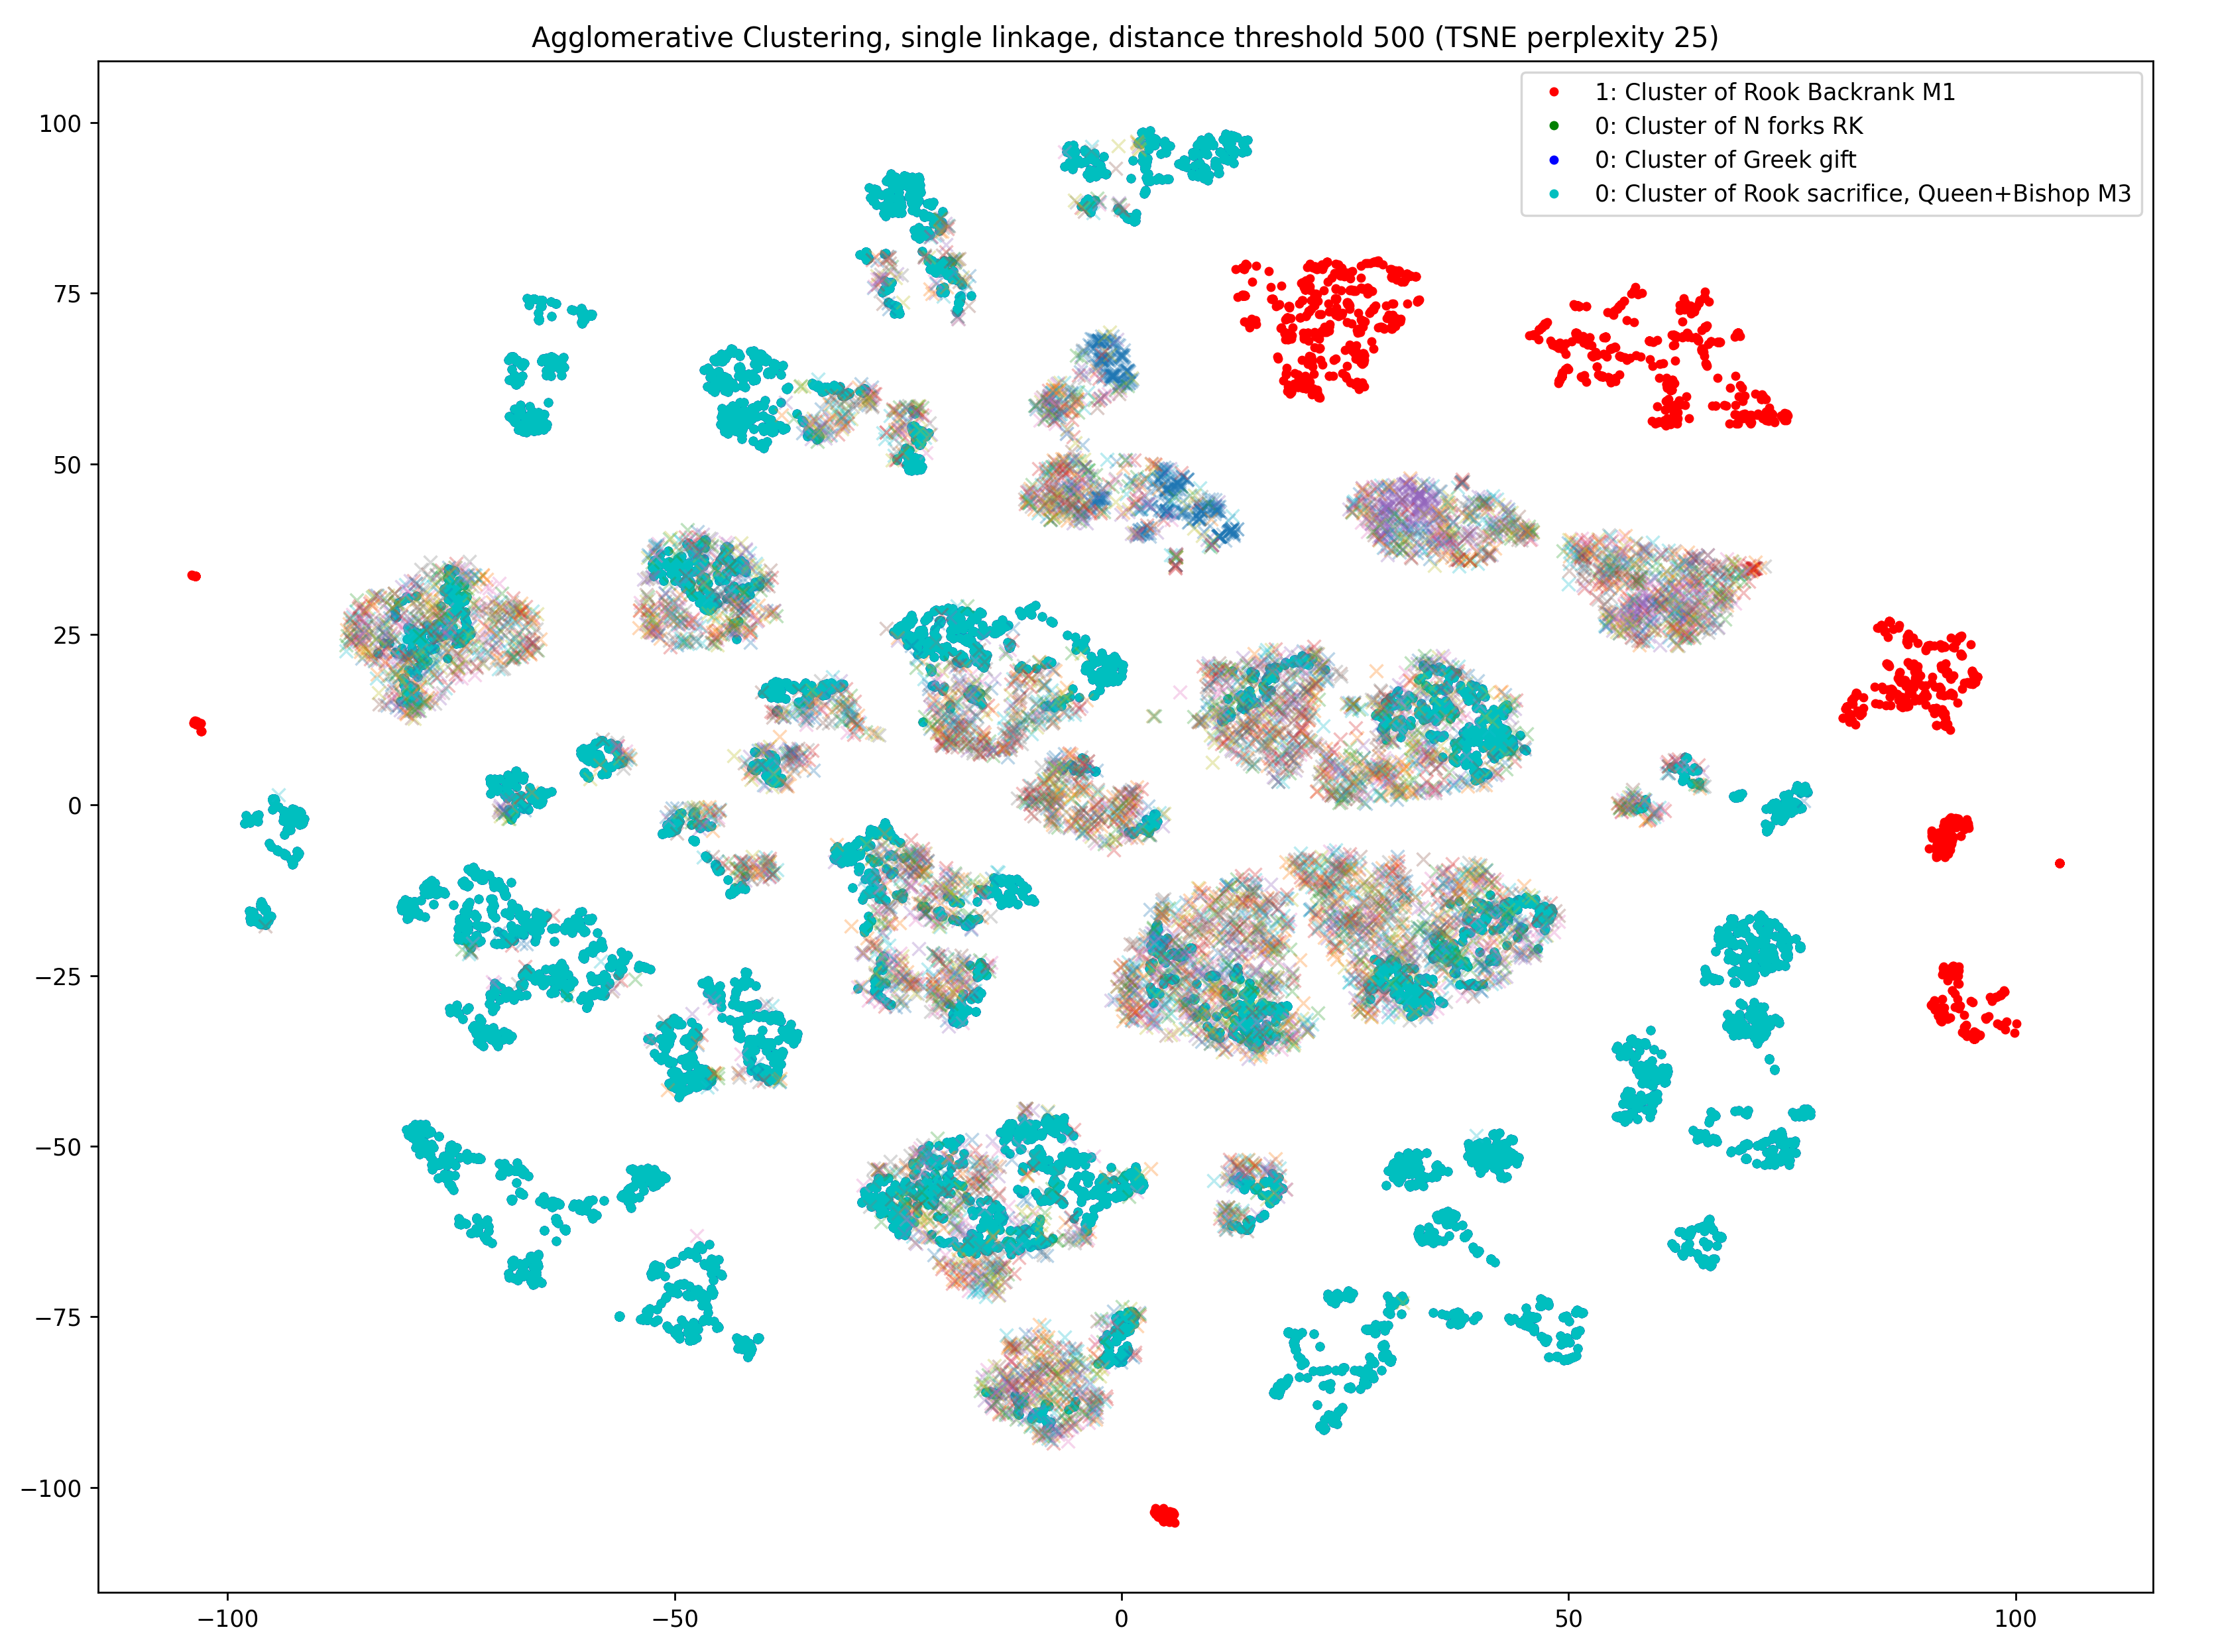
\includegraphics[width=0.9\textwidth]{project/img/tsne/ac_25.png}
  \caption{Agglomerative Clustering (single linkage, distance threshold $500$)}
  \label{tsne1}
\end{figure}

\begin{figure}[H]
  \centering
  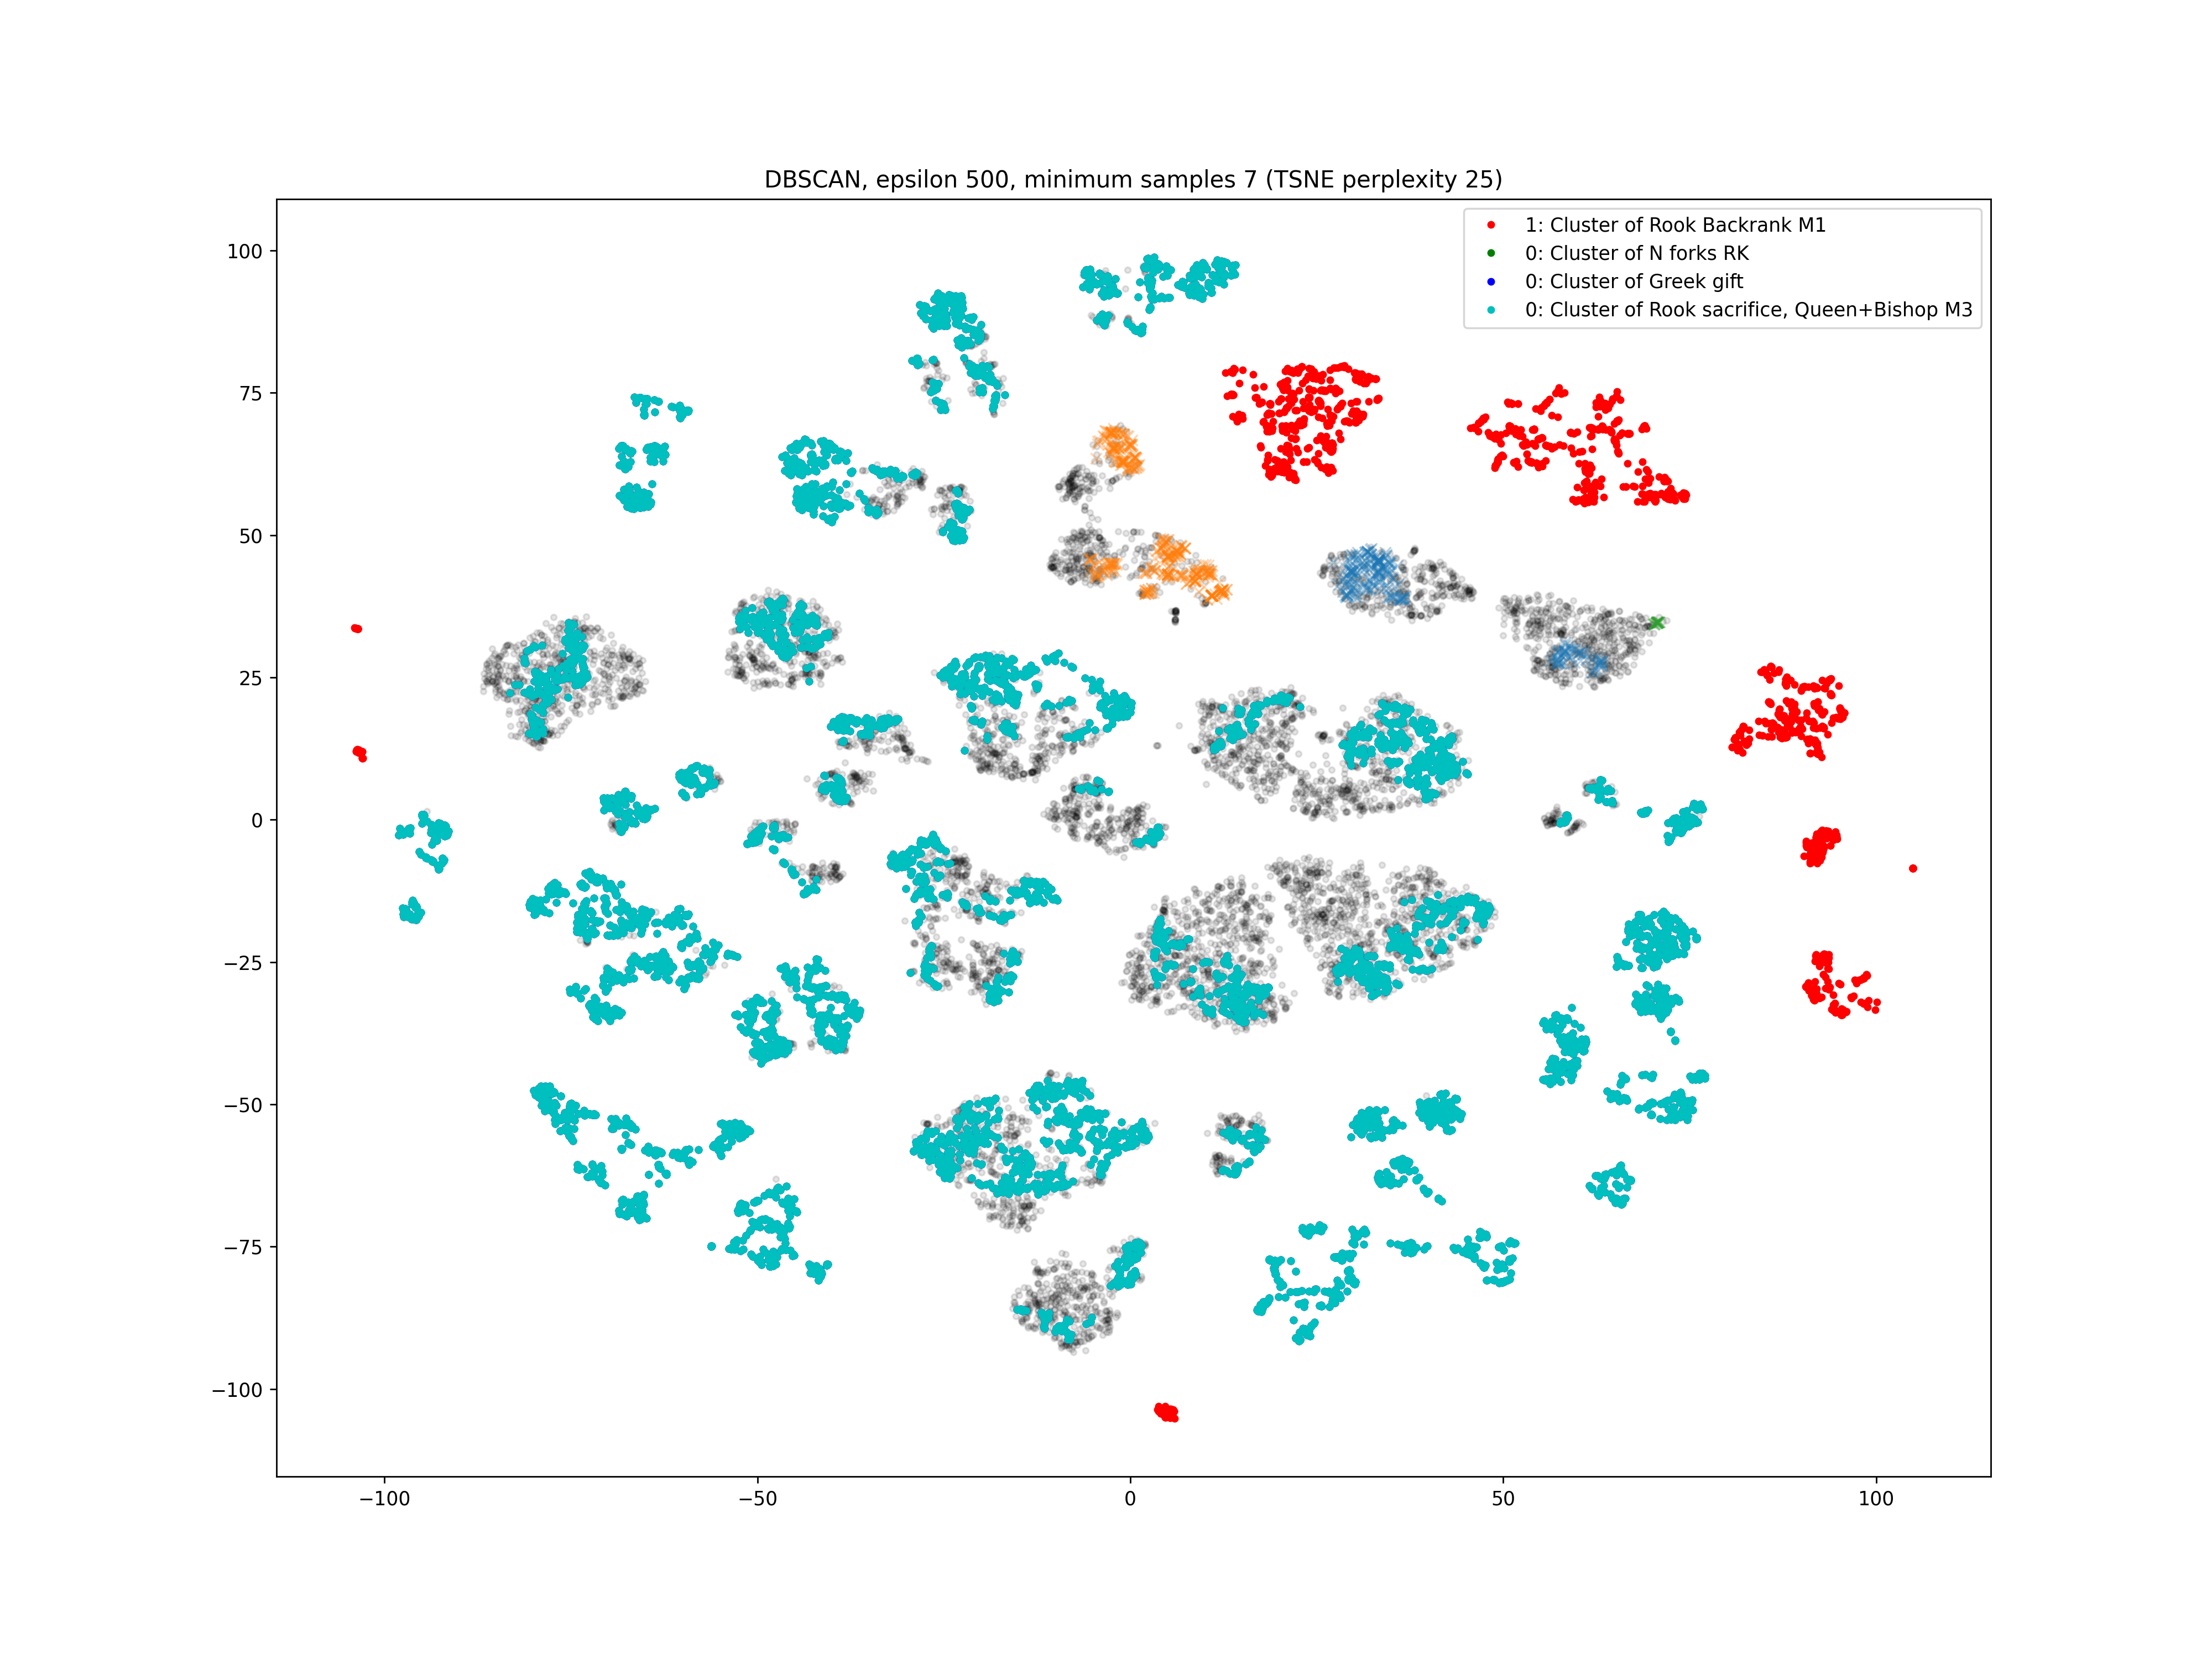
\includegraphics[width=0.9\textwidth]{project/img/tsne/dbscan_500_25.png}
  \caption{DBSCAN, $\epsilon=500$, minimum samples $7$.}
  \label{tsne2}
\end{figure}

\begin{figure}[H]
  \begin{minipage}[t]{0.475\textwidth}
    \centering
    \chessboard[setfen= 2rr2k1/ppb3pp/8/3p1q2/1P1Qn2P/P2KP2p/1B6/2RR4 w - -
    2 32]
    \caption{Puzzle in the same cluster as the \emph{back-rank mate-in-one}
    puzzle (\Cref{chess11}). Solution: \texttt{1.Qxg7\#}}
    \label{dbscanCluster11}
  \end{minipage}
  \hspace{0.05\textwidth}
  \begin{minipage}[t]{0.475\textwidth}
    \centering
    \chessboard[setfen= r3k2r/pp1qbppp/2pp1n2/8/3QP3/2N2P1P/PPP2P2/R1B3RK b
    kq - 4 13]
    \caption{Puzzle in the same cluster as the \emph{back-rank mate-in-one}
    puzzle (\Cref{chess11}). Solution: \texttt{1...Qxh3\#}}
    \label{dbscanCluster12}
  \end{minipage}
\end{figure}

\begin{figure}[H]
  \begin{minipage}[t]{0.475\textwidth}
    \centering
    \chessboard[setfen=8/8/1p3k2/p6p/P3K1pP/1P4P1/8/8 w - - 5 46]
    \caption{Puzzle from the endgame cluster. Both sides' pawns are frozen:
    they are either unable to move, or moving would cause them to be captured,
    creating a passed pawn for the opponent and losing the game. White wins
    with \texttt{1.Kf4}, getting \emph{opposition}, shouldering the black king
    away from the \texttt{h5} pawn.}
    \label{dbscanCluster13}
  \end{minipage}
  \hspace{0.05\textwidth}
  \begin{minipage}[t]{0.475\textwidth}
    \centering
    \chessboard[setfen=5k2/1N3ppp/n3p3/P7/5P2/6P1/7P/6K1 b - - 0 33]
    \caption{Puzzle from the endgame cluster. \texttt{1...Ke7} traps the
    knight(!), which is captured by the black king a few moves later.}
    \label{dbscanCluster14}
  \end{minipage}
\end{figure}

\begin{figure}[H]
  \centering
  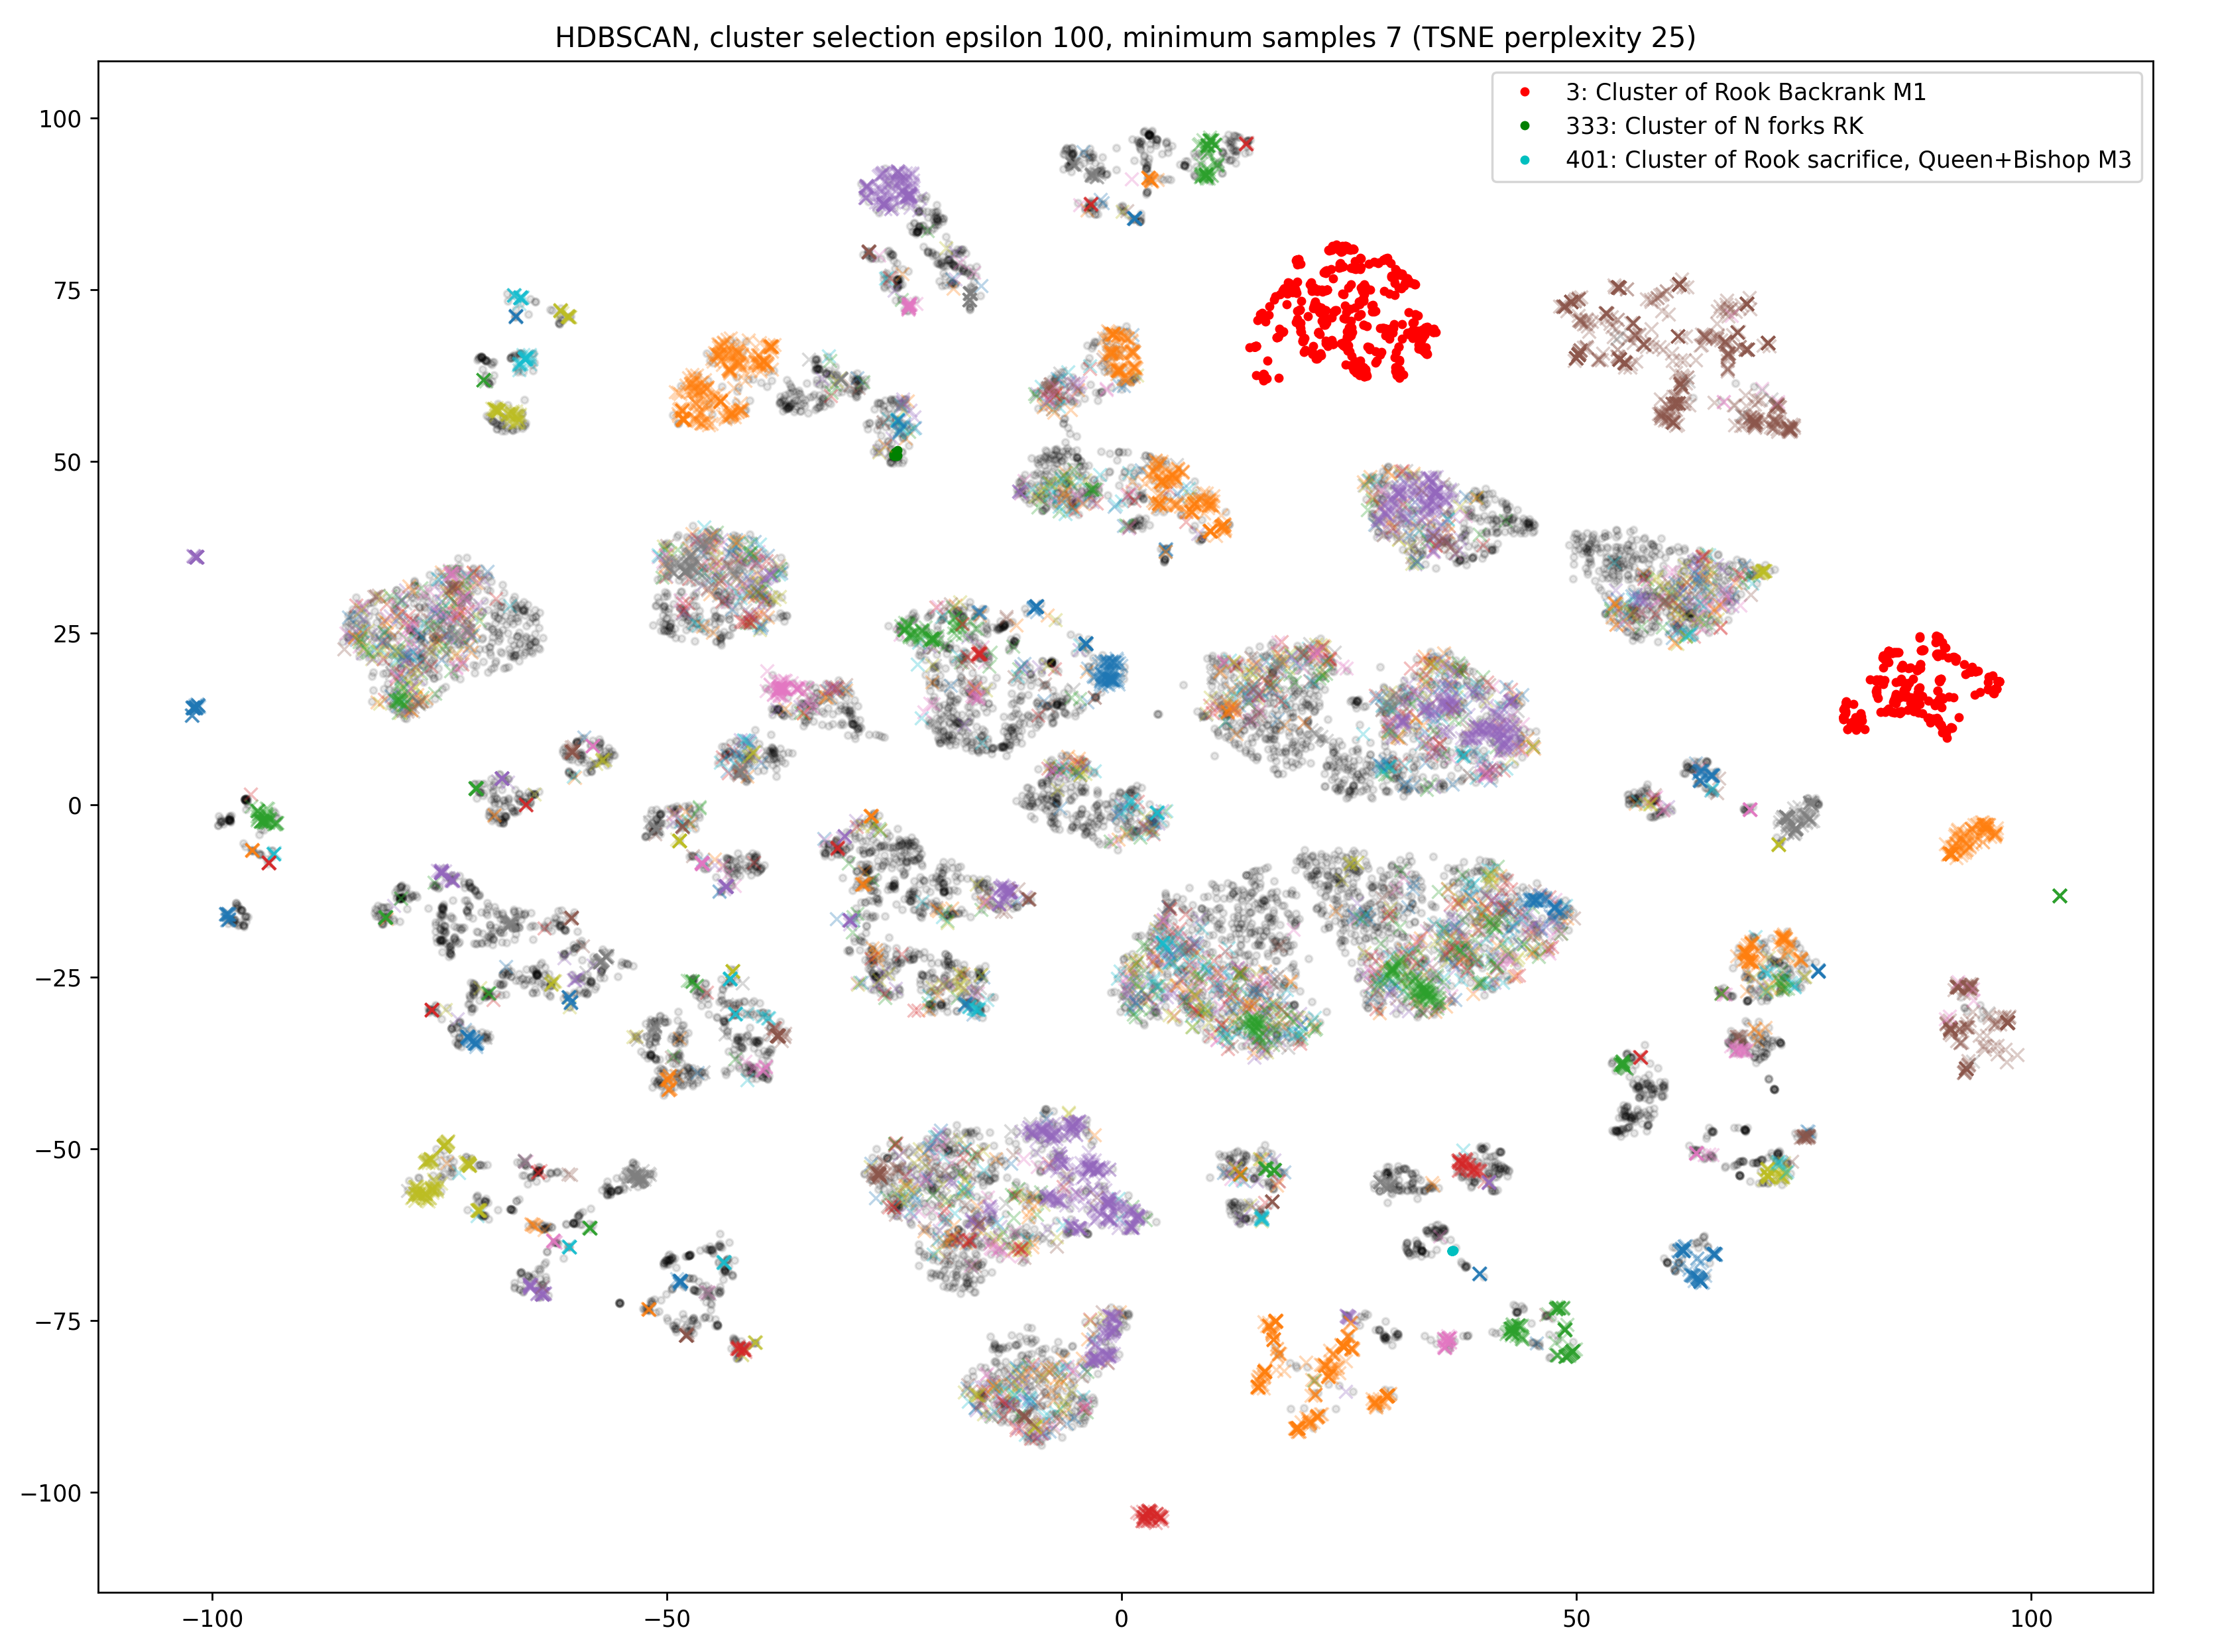
\includegraphics[width=0.8\textwidth]{project/img/tsne/hdbscan_2_25.png}
  \caption{HDBSCAN, cluster selection $\epsilon=100$, minimum samples $7$.}
  \label{tsne3}
\end{figure}

HDBSCAN puzzle clustering (\Cref{tsne3}), breaks up the megacluster which was
apparent in the previous two examples, and there are a few promising clusters.
In total, there are 420 clusters, with a mean cluster size of $22.82$.
Unfortunately, the \emph{Greek gift} puzzle (\Cref{chess13}) is outside of any
clusters, which is surprising, given the apparent effectiveness of this
algorithm.

Despite this, the clustering seems to perform much better than the former
attempts, and yields useful results. Cluster 333, under which the \emph{knight
fork} puzzle (\Cref{chess12}) falls, contains 18 puzzles, of which 17 are
tagged with `short' and 15 with `fork'. Two further puzzles are taken from this
cluster (\Cref{hCl1,hCl2}). Interestingly, the puzzle in \Cref{hCl2} is
not tagged as a `fork', even though it undeniably forks the king and bishop.
The remaining puzzles with no `fork' tag in this cluster have been manually
checked and are indeed knight forks. This is a good result, as it shows that
this method can pick up on themes that the Lichess puzzle database missed.

Another cluster of 61 puzzles was also found, 56 of which are tagged as
`endgame', a further 37 as `rook endgame', and none feature a `mate'. This
cluster appears to contain various rook and pawn endgames, where the opposing
side offers a rook trade. Accepting the trade is the only winning move for the
side solving the puzzle, and this cluster contains the puzzles with this theme.
An easy example (\Cref{chess15}) and a complex example (\Cref{chess16}) from
this cluster are featured.

These clusters are very interesting to analyse, as this method can pick up on
puzzle similarity that is not immediately obvious. During experimentation, it
was found that a larger distance matrix drastically improves the clustering
performance; this is likely because there are more examples of niche tactical
patterns, which means they can be clustered together. Without enough examples,
many of these puzzles are categorised as as noise/outliers: approximately 50\%
(\Cref{tabHDBSCAN}). 

If a larger distance matrix can be constructed, it is likely that the
clustering method will improve more, and allow finer categorisation of puzzles.
The resource and time commitment to do so unfortunately prohibited this.

\begin{figure}[H]
  \begin{minipage}[t]{0.475\textwidth}
    \centering
    \chessboard[setfen=3r2r1/PR6/2pk2p1/1p1p1nP1/3PnPQ1/1PP1P3/2K5/5R2 b -
    - 0 39]
    \caption{Puzzle from the \emph{knight fork} cluster. Black forks with
    \texttt{1...Nxe3+}, hitting two major pieces at once.}
    \label{hCl1}
  \end{minipage}
  \hspace{0.05\textwidth}
  \begin{minipage}[t]{0.475\textwidth}
    \centering
    \chessboard[setfen=
    rn1q1b1r/pp3kpp/2p2n2/4p3/4p1b1/2NP1N2/PPP2PPP/R1BQK2R w KQ - 0 8]
    \caption{Puzzle from the \emph{knight fork} cluster. White wins a bishop
    after \texttt{1.Nxe5+}.}
    \label{hCl2}
  \end{minipage}
\end{figure}

\begin{figure}[H]
  \begin{minipage}[t]{0.475\textwidth}
    \centering
    \chessboard[setfen=8/8/k5r1/p5R1/5K2/P7/8/8 b - - 1 51]
    \caption{Rook trade cluster. After \texttt{1...Rxg5 2.Kxg5 Kb5}, Black wins
    the remaining white pawn and shoulders the white king for a victory.}
    \label{chess15}
  \end{minipage}
  \hspace{0.05\textwidth}
  \begin{minipage}[t]{0.475\textwidth}
    \centering
    \chessboard[setfen=8/2p4p/1k4p1/p1r5/2R4P/1P2K3/P4P2/8 b - - 3 47]
    \caption{Complex position in the rook trade cluster. \texttt{1...Re5+} is
    tempting, and was played in the game where this position occured. This,
    however, loses the advantage. After trading rooks, \texttt{1...Rxc4
    2.bxc4}, Black threatens to win the \texttt{c4} pawn with \texttt{2...Kc5
    3.Kd3 Kb4}, allowing Black to capture the \texttt{a2} pawn. The white king
    cannot trap the black king on the \texttt{a} file as both sides quickly run
    out of pawn moves. With correct play, White is forced into
    \emph{zugzwang}.}
    \label{chess16}
  \end{minipage}
\end{figure}

\pagebreak

\section{$k$-Nearest Neighbours}\label{treeS3}

Since the unsupervised clustering method (\Cref{treeS2}) produces too many
outliers to be useful for inference, a classic $k$-nearest neighbours ($k$-NN)
approach \citep{fix1985discriminatory} can be used both for classification of
puzzle themes and regression of puzzle difficulty rating.

It has been shown that the novel distance function (\Cref{treeS13}) has
promising results for finding similar positions to a given puzzle
(\Cref{treeS21}), so with the appropriate setup, this method should be viable
for inference and comparison to the deep learning (\Cref{mlChapter}) method.

\subsection{Label Prediction and Difficulty Regression with $k$-NN}

The process of predicting a label and difficulty for an unseen chess puzzle is
straightforward. Given a puzzle, its $k$ nearest neighbours in the known
(training) dataset are found. If half or more of the neighbours are tagged with
a certain tactic label, the puzzle is predicted to have that label. The puzzle
difficulty is the mean of the difficulty of the neighbours.

\subsection{Search for the Best $k$}\label{treeS31}

One of the downsides of $k$-NN is the slow inference performance. This makes
tuning the parameter $k$ difficult, as the running time is roughtly
proportional to the multiple of the training set size and validation set size.
To address this, random subsets of the training and validation sets
(\Cref{mlS12}) of size 20,000 each were used. This amount showed acceptable
clustering performance (\Cref{treeS22}), so it will provide a reasonable
starting point for this approach.

Paramater $k$ was varied from $1$-$100$. The results (\Cref{knn}) show that
$k=24$ is optimal for label prediction, with an average of $2.8011$ incorrect
labels (includes both false positives and false negatives). For difficulty
regression, $k=22$ is best, with an average mean squared difficulty rating
error of $\sim\!434.0^2$. 

Even though different $k$ values for the two tasks are possible, $k=24$ was
chosen for both, as it simplifies implementation and increases difficulty
regression error to $\sim\!434.3^2$ -- a negligible difference. 

\begin{figure}[H]
  \centering
  
\includegraphics[width=0.9\textwidth]{project/img/knn.png}
  \caption{Effect of $k$ on label prediction and difficulty regression performance.}
  \label{knn}
\end{figure}

